\documentclass[11pt]{aghdpl}
\usepackage[english]{babel}
\usepackage[utf8]{inputenc}

\usepackage{mathtools}
\usepackage{amsfonts}
\usepackage{amsmath}
\usepackage{amsthm}
\usepackage{qtree}
\usepackage{tikz}
\usepackage{tikz-qtree}
\usepackage{etoolbox}
\usepackage{enumerate}
\usepackage{setspace}
\usepackage{url}
\usepackage{enumitem}
\usepackage{adjustbox}

% \linespread{1.25}
% --- < bibliografia > ---


\usepackage[
style=numeric,
sorting=none,
%
% Zastosuj styl wpisu bibliograficznego właściwy językowi publikacji.
language=autobib,
autolang=other,
% Zapisuj datę dostępu do strony WWW w formacie RRRR-MM-DD.
urldate=iso
% Nie dodawaj numerów stron, na których występuje cytowanie.
backref=false,
% Podawaj ISBN.
isbn=true,
% Nie podawaj URL-i, o ile nie jest to konieczne.
url=true,
% Ustawienia związane z polskimi normami dla bibliografii.
maxbibnames=3,
% Jeżeli używamy BibTeXa:
backend=bibtex
]{biblatex}

\usepackage{csquotes}
\newtheorem{example}{Przyklad}[section]
% Ponieważ `csquotes` nie posiada polskiego stylu, można skorzystać z mocno zbliżonego stylu chorwackiego.
\DeclareQuoteAlias{croatian}{polish}



% Użyj czcionki kroju Courier.
\usepackage{courier}

\usepackage{listings}
\lstloadlanguages{TeX}

\lstset{
	literate={ą}{{\k{a}}}1
           {ć}{{\'c}}1
           {ę}{{\k{e}}}1
           {ó}{{\'o}}1
           {ń}{{\'n}}1
           {ł}{{\l{}}}1
           {ś}{{\'s}}1
           {ź}{{\'z}}1
           {ż}{{\.z}}1
           {Ą}{{\k{A}}}1
           {Ć}{{\'C}}1
           {Ę}{{\k{E}}}1
           {Ó}{{\'O}}1
           {Ń}{{\'N}}1
           {Ł}{{\L{}}}1
           {Ś}{{\'S}}1
           {Ź}{{\'Z}}1
           {Ż}{{\.Z}}1,
	basicstyle=\footnotesize\ttfamily,
}

\AtBeginDocument{
	\renewcommand{\tablename}{Table}
	\renewcommand{\figurename}{Fig.}
}

% ------------------------
% --- < tabele > ---
\usepackage{array}
\usepackage{tabularx}
\usepackage{multirow}
\usepackage{booktabs}
\usepackage{makecell}
\usepackage[flushleft]{threeparttable}

% defines the X column to use m (\parbox[c]) instead of p (`parbox[t]`)
\newcolumntype{C}[1]{>{\hsize=#1\hsize\centering\arraybackslash}X}

%%%%%%%%%%%%%%%%%%%%%%%%%%%%%%%%%%%%%%%%%%%%%%%%%%%%%%%%%%%%
\author{Dawid Talaga}
\shortauthor{D. Talaga}

\titlePL{Niespójności niekompletnych macierzy porównań parami}
\titleEN{Inconsistency of incomplete pairwise comparisons matrices}

\shorttitlePL{Niespójności niekompletnych macierzy porównań parami}
\shorttitleEN{Inconsistency of incomplete pairwise comparisons matrices}

\thesistype{Master of Science Thesis}
\supervisor{Konrad Kułakowski PhD}

\degreeprogramme{Computer Science}
\date{2018}
\department{Department of Applied Computer Science}

\faculty{Faculty of Electrical Engineering, Automatics,\protect\\[-1mm] Computer Science and Biomedical Engineering}

\acknowledgements{Serdecznie dziękuję Promotorowi Panu dr. hab. Konradowi Kułakowskiemu za zainteresowanie mnie tematem PC oraz życzliwe wsparcie.\\
Dziękuj̨ę moim Rodzicom, dzięki którym mogłem rozwijać się i studiować oraz bliskim mi osobom, które dodawały mi wiary w moje siły.}

\setlength{\cftsecnumwidth}{10mm}
\brokenpenalty=10000\relax


%---------------------------------------------------------------------------
\setcounter{secnumdepth}{4}
\brokenpenalty=10000\relax

\addbibresource{bibliografia.bib}

\begin{document}

\titlepages

\fancypagestyle{plain}
{
	\fancyhf{}
	\renewcommand{\headrulewidth}{0pt}
	\renewcommand{\footrulewidth}{0pt}
}

% \pagestyle{empty}
\setcounter{tocdepth}{2}
\tableofcontents
\clearpage

\chapter{Introduction}
\label{cha:wprowadzenie}

\section{Pairwise Comparisons method}
\label{sec:metodaPorowan}
People have made decisions for ages. Some of them are very simple and come easily but others, more complicated, require deeper analysis. It happens when there are many compared objects, which are complex and the selection criterion is hard to measure precisely. Fortunately, the development of mathematics brought an interesting tool - \textit{The Pairwise Comparisons (PC) Method}. The first case of using the method (in a very simple version) is the election system described by Ramond Llull \cite{Colomer2013} in the thirteenth century. Its rules were based on the fact that the candidates were pairwise compared with each other and the winner was the one who won in the largest number of direct comparisons. The method was reinvented in the eighteenth century by Condorcet and Bord \cite{Kulakowski2016} as they proposed it in their voting system. In the twentieth century, the method found the application in the theory of social choice, the main representatives of which were the Nobel prize winners Keneth Arrow \cite{Arrow} and Amartya Sen \cite{Sen}. The current shape of the method was influenced by the changes introduced by Fechner \cite{Fechner1966} and then refined by {Thrustone} \cite{Thurstone1994}. However, the breakthrough was the introduction to the method \textit\textit{The Analytic Hierarchy Process (AHP)} by Saaty \cite{Saaty2008}, which allowed to compare many more complex objects and create a hierarchical structure.The primary aim of this paper is to check which method of calculating the inconsistency is the best in this case. In order to do it, a series of tests were carried out on various known inconsistency indexes, taking into account many different parameters: the matrix size, the amount of missing data and the level of inconsistency. The results of the research are included in this paper.

The PC method is based on the assumption that it is not worth comparing all objects at the same time. It is better to compare them in pairs and then gather the results together. Such pairwise comparisons are much more intuitive and natural for a human being. How can one be sure that these judgments are consistent? Or what to do if some comparisons are missing? In such a case, is it worth taking the PC method at all?

The answer to the first question is the concept of inconsistency introduced into the method. This paper tries to answer the next two questions - meaning to examine whether available methods for determining inconsistencies give reliable results when a part of the comparisons is missing. 

\section{The aim of the work}
\label{sec:celePracy}
The main aim of this paper is to check which method of calculating the inconsistency is the best when some comparisons are missing. In order to do so, a series of tests was carried out on various known inconsistency indexes, taking into account many different parameters: the matrix size, the amount of missing data and the level of inconsistency.
The tests were implemented in the \textit{R} language which properly fit into numerical calculations.

It was not known from the beginning what the result of this work would be. It was considered that one or more existing inconsistency indexes would turn out to be appropriate for incomplete matrices also or that the tests would show that the inconsistency could not be calculated by these indexes. 
The results of the research are included in this study.

\section{Content of the work}
\label{sec:zawartoscPracy}
The work includes the theoretical part and the description of conducted experiments and their results. It consists of six chapters.\\
The second chapter shows the Pairwise Comparisons method and the problem of inconsistency. Understanding the basics is necessary to go into the further chapters.\\
In the third chapter, sixteen available methods for calculating the inconsistency for the PC matrices are presented. \\
The fourth chapter shows ideas which allow to perform tests. These are modifications of existing inconsistency indexes which enable to adjust them to incomplete matrices and the algorithm which tests the quality of the modified indexes. \\
The results of experiments are presented and discussed in the fifth chapter.\\
The last chapter contains summary, conclusions and ideas for future researches.
\chapter{Pairwise Comparisons method}
\label{sec:pcMethod}
  \section{PC matrix}
	\label{subsec:macierzPC}
	
	The \textit{PC method} is used to choose the best alternative from a set of concepts. However, this goal is achieved by comparing in pairs. A numerical value is assigned to each pair. It not only determines which alternative is preferred but also informs about the strength of this preference. In this way, the finite set of concepts $C=\left\{ c_{1},\ldots,c_{n}\right\} $ is transformed into a \textit{PC matrix} $M=\left(m_{ij}\right)$, where $m_{i,j}\in \mathbb{R}$ and $i,j\in\left\{ 1,\ldots,n\right\}$. The PC matrix for $n$ concepts is following:
$$
M = 
\left(
\begin{array}{lllll}
	1 & m_{12} & \dots & m_{1n}\\
	m_{21} & 1 & \dots & m_{2n}\\
	\vdots & \vdots & \ddots & \vdots\\
	m_{n1} & m_{n2} & \dots & 1\\ 	
\end{array}
\right)
$$

	It is worth noting that the values $m_{ij}$ and $m_{ji}$ represent the same pair. Therefore, one should expect that $m_{ji}=\frac{1}{m_{ij}}$. If
	\begin{equation} 
		\forall _{i,j\in\left\{ 1,\ldots,n\right\}} :m_{ij}=\frac{1}{m_{ji}},
	\end{equation}
		the matrix is called a \textit{reciprocal}.

  \section{Weight vector}
	\label{subsec:wektorWag}
	
	The PC matrix is the basis for calculating the method. It is used in a function $\mu:C\rightarrow \mathbb{R}$ that assigns a positive real number to each alternative in the set $C$. The vector $$\mu=\left[\mu\left(c_{1}\right),\ldots,\mu\left(c_{n}\right)\right]$$ formed in this way is called \textit{the weight vector} or \textit{the priority vector} (see Fig.2.1). It informs which alternative won.

\begin{figure}[ht]
\centerline{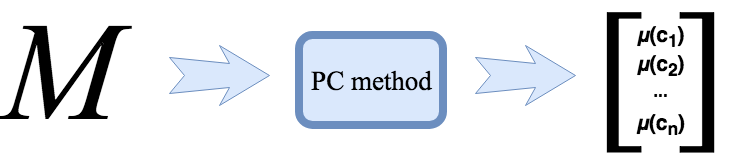
\includegraphics[scale=2.5]{fig1.png}}
\caption{Diagram of calculating \textit{the weight vector} based on the article \cite{Kulakowski2014}}
\end{figure}

There are many ways to calculate the vector $\mu$. Among the popular ones are the method using the matrix's eigenvalues or the method based on geometric means \cite{SAATY1998}.

\section{Inconsistency}
\label{subsec:inconsistency}
The second important parameter describing the PC matrix is \textit{consistency}. The matrix is consistent if 
	\begin{equation}
		\label{eq:consistent}
		\forall _{i,j,k \in\left\{ 1,\ldots,n\right\}} :m_{ik}=m_{ij}m_{jk}.
	\end{equation}
Three numbers that should meet this assumption are called a \textit{triad}.

If the matrix is consistent and the weight vector $\mu$ is computed, then for each of the variables $i,j$, where $1\leq i,j\leq n$ meets the equation: 
	\begin{equation} 
		\label{eq:consistent2}		
		m_{ij}=\frac{\mu_{i}}{\mu_{j}}.
 	\end{equation}
In practice, it is very rare for a matrix $M$ to be completely consistent. In the long history of the PC method, many methods were developed to calculate inconsistencies. Many of them are based directly on the definition of consistency~\ref{eq:consistent}, some methods use the eigenvalues of the matrix, others are based on the assumption that each fully consistent matrix fulfills the condition~\ref{eq:consistent}.
\chapter{Inconsistency indexes}
\label{sec:inconsistencyIndexes}
\section{Inconsistency indexes for complete matrices}

This subsection presents sixteen common inconsistency indexes. Their detailed description, including the formulas, is necessary to modify them in the next step so that they can also work for incomplete matrices. Many of them were described and tested numerically in article \cite{Brunelli2013}. In all methods, it is assumed that the PC matrix is reciprocal.


 \subsection{Saaty index ($CI$)}

This is one of the most important and popular indexes and was introduced by Saaty \cite{SAATY1977}. In order to determine inconsistency, the matrix's eigenvalues should be computed. The author used the dependence that the largest eigenvalue of the matrix is equal to its dimension if and only if the given matrix is completely consistent. On this assumption, he based his thoughts and proposed the formula:
	\begin{equation} 
		CI(M)=\frac{\lambda_{max}-n}{n-1},
	 \end{equation}
 where $\lambda_{max}$
  is the principal eigenvalue of the PC matrix and $n$
  is its dimension.


\subsection{Geometric consistency index ($GCI$)}

This index on the assumption ~\ref{eq:consistent2} was proposed by Craford and Williams \cite{CRAWFORD1985} and then refined by Aguaròn and Moreno-Jimènez \cite{AGUARON2003}. In this case the priority vector should be calculated using the geometric mean method. Consider~\ref{eq:consistent} one can create a matrix:
	\begin{equation} 
		E=\left[e_{ij}\mid e_{ij}=m_{ij}\frac{w_{j}}{w_{i}}\right],\,\,\,\,\,\,i,j=1,...,n.
	 \end{equation}
 The inconsistency index is calculated as follows:
	 \begin{equation} 
		\label{eq:GCI}
		GCI=\frac{2}{(n-1)(n-2)}\sum_{i=1}^{n}\sum_{j=i+1}^{n}ln^{2}e_{ij}.
	 \end{equation}
 

\subsection{Koczkodaj index ($K$)}

One of the most popular inconsistency indexes was proposed by Koczkodaj \cite{KOCZKODAJ1993}. It is based directly on the definition of consistency~\ref{eq:consistent}. The value of the inconsistency index for one triad triad was defined as:
	\begin{equation} 
		\label{eq:K}
		K_{i,j,k}=min\{\frac{1}{m_{ij}}\mid m_{ij}-\frac{m_{ik}}{m_{jk}}\mid,\frac{1}{m_{ij}}\mid m_{ik}-m_{ij}m_{jk}\mid,\frac{1}{m_{jk}}\mid m_{jk}-\frac{m_{ik}}{m_{ij}}\mid\}.
	 \end{equation}

 This formula was simplified by Duszak and Koczkodaj \cite{DUSZAK1994} and is given as:
 	\begin{equation} 
		K(\alpha,\beta,\gamma)=min\{\mid1-\frac{\beta}{\alpha\gamma}\mid,\mid1-\frac{\alpha\gamma}{\beta}\mid\},\,\,\,\,\,\,where\,\alpha=m_{ij},\beta=m_{ik},\gamma=m_{jk}
	 \end{equation}
 Then it was generalized \cite{DUSZAK1994} for $n>2$. Finally, the inconsistency index has the following form:
 	\begin{equation} 
		K=max\{K(\alpha,\beta,\gamma)|1\leq i<j<k\leq n\}.
	 \end{equation}
 It is worth noting that not only does the coefficient find the greatest inconsistency but also indicates the place in which it occurs.


\subsection{Kazibudzki indexes ($MLTI, MLTI^{*}, CMLTI*$)}

Based on the Koczkodaj inconsistency index and observation that $ln(\frac{\alpha\gamma}{\beta})=-ln(\frac{\beta}{\alpha\gamma})$, Kazibudzki proposed several additional inconsistency indexes \cite{Kazibudzki2016}. Instead of the formula for inconsistency of the triad [eq:k-abg], he introduced two new formulas:
	\begin{equation} 
		LTI(\alpha,\beta\gamma)=\mid ln(\frac{\alpha\gamma}{\beta})\mid,
	 \end{equation}
	\begin{equation}
		\label{eq:lti*} 
		LTI*(\alpha,\beta\gamma)=ln^{2}(\frac{\alpha\gamma}{\beta}).
	 \end{equation}
Based on the above equations, Kazibudzki proposed new indexes. The simplest ones use the geometric mean of the triads. Thus, new indexes could be written in the form:
	\begin{equation} 
		MLTI(LTI)=\frac{1}{n}\sum_{i=1}^{n}\left[LTI_{i}(\alpha,\beta\gamma)\right],
	 \end{equation}
 	\begin{equation} 
		MLTI(LTI*)=\frac{1}{n}\sum_{i=1}^{n}\left[LTI*_{i}(\alpha,\beta\gamma)\right].
			 \end{equation}
 

After further research Kazibudzki introduces another inconsistency index \cite{Kazibudzki2017}, again based on~\ref{eq:lti*}. It was defined as $CM(LTI*)=\frac{MEAN[LTI*(\alpha,\beta,\gamma)]}{1+MAX[LTI*(\alpha,\beta,\gamma)]}$. Hence,
	\begin{equation} 
		CM(LTI*)=\frac{\frac{1}{n}\sum_{i=1}^{n}[LTI*_{i}(\alpha,\beta,\gamma)]}{1+max\{LTI*_{i}(\alpha,\beta,\gamma)\}}.
	 \end{equation}
 

\subsection{Index of determinants ($PL$)}

This index was proposed by Pelaez and Lamata \cite{PELAEZ2003} and is also based on the concept of triad. The authors noticed that PC  matrices can be constructed on the basis of triads. Their determinant is closely related to the consistency of the matrix.

For every triad $(m_{ik},m_{ij},m_{jk})$ one can build a matrix in the form: 
	\begin{equation} 
		T_{ijk}=\left(\begin{array}{ccc}
			1 & m_{ij} & m_{ik}\\
			\frac{1}{m_{ij}} & 1 & m_{jk}\\
			\frac{1}{m_{ik}} & \frac{1}{m_{jk}} & 1
		\end{array}\right),\,\,\,\,\,\,where\,i<j<k.
	\end{equation}
 The determinant of this matrix is:
	\begin{equation} 
		det(M)=\frac{m_{ik}}{m_{ij}m_{jk}}+\frac{m_{ij}m_{jk}}{m_{ik}}-2.
	 \end{equation}
 If the matrix is fully consistent, then $det(M)=0$, else $det(M)>0$. Based on the above considerations, the authors introduced the new inconsistency index that can be formulated as follows:
 	\begin{equation} 
		CI*=\frac{1}{n}\sum_{i=1}^{n}\left(\frac{m_{ik}}{m_{ij}m_{jk}}+\frac{m_{ij}m_{jk}}{m_{ik}}-2\right).
	 \end{equation}
 

\subsection{Kułakowski and Szybowski indexes ($I_1, I_2, I_{\alpha}, I_{\alpha,\beta}$ ) }

Kułakowski and Szybowski proposed two further inconsistency indexes \cite{KULAKOWSKI20141}, which are also based on triads. They use the fact that the number of triads that can be found in a PC matrix is:
	\begin{equation} 
		\label{eq:nPo3}
		\binom{n}{3}=\frac{n!}{(n-3)!3!}=\frac{n(n-1)(n-2)}{6}.
	 \end{equation}
 The index is formulated as follows:
	 \begin{equation} 
	 \label{eq:I1}		
		I_{1}=\frac{6\sum_{t\in T}K(t)}{n(n-1)(n-2)},
	 \end{equation}
 where $K(t)$ is the Koczkodaj index for triad $t=(\alpha,\beta,\gamma)$ of the set of all triads $T$. 

The second inconsistency index is similar:
	\begin{equation} 
	 \label{eq:I2}				
		I_{2}=\frac{6\sqrt{\sum_{t\in T}K^{2}(t)}}{n(n-1)(n-2)}.
	 \end{equation}

Indexes can be combined with each other to create new coefficients. In this way Kułakowski and Szybowski proposed two new indexes. The first one is based on~\ref{eq:K} and~\ref{eq:I1}. This index allows to choose which value should have more impact on the result: the greatest inconsistency found or the average inconsistency of all triads. The new inconsistency index looks as follows:
	\begin{equation} 
		I_{\alpha}=\alpha K+(1-\alpha)I_{1},
	 \end{equation}
 where $0\leq\alpha\leq1$.
  
The second index expands the first one by~\ref{eq:I2}:
	\begin{equation} 
		I_{\alpha,\beta}=\alpha K+\beta I_{1}+(1-\alpha-\beta)I_{2}.
	 \end{equation}
 

\subsection{Harmonic consistency index ($HCI$)}

This index was introduced by Stein and Mizzi and it presents a completely new method of inconsistency computing \cite{STEIN2007}. At the beginning it requires the creation of an auxiliary vector $s=(s_{1},...,s_{n})^{T}$, where $n$ is the dimension of the matrix $M$, for which the index will be calculated. Each element of the vector $s$ is the sum of values in one column of the matrix $M$. Hence, 
	\begin{equation} 
		s_{j}=\sum_{i=1}^{n}m_{ji}\,\,\,\,\,\,\forall j.
	 \end{equation}
 The authors proved that if the matrix $M$ is consistent, then $\sum_{j=1}^{n}s_{j}^{-1}=1$. The formula for the mean harmonic looks as follows (Brunelli, 2015):
	 \begin{equation} 
		\label{eq:hm1}
		HM=\frac{n}{\sum_{j=1}^{n}\frac{1}{s_{j}}}.
	 \end{equation}
 The final formula for the inconsistency index was obtained by normalizing the above equation~\ref{eq:hm1}:
 	\begin{equation} 
		HCI=\frac{\left(HM(s)-n\right)\left(n+1\right)}{n(n-1)}.
	 \end{equation}
 

\subsection{Golden and Wang index ($GW$)}

This index was introduced by Golden and Wang \cite{Golden1989}. It assumes that the priority vector was calculated using the geometric mean method, then normalized to add up to $1$. In this way vector $g*=[g{}_{1,}^{*},...,g_{n}^{*}]$ was obtained, where $n$ is the dimension of the matrix $M$. The next step is to normalize each column of the matrix $M$. After this, the sum of the elements of each column in matrix $M$ is $1$. The obtained matrix is marked with the symbol $M^{*}$. The inconsistency index is defined as follows:
	\begin{equation} 
		GW=\frac{1}{n}\sum_{i=1}^{n}\sum_{j=1}^{n}\mid m_{ij}^{*}-g_{i}^{*}\mid.
	 \end{equation}
 

\subsection{Salo and Hamalainen index ($CM$)}

The index proposed by Salo and Hamalainen \cite{SALO1995} uses the definition of inconsistency~\ref{eq:consistent}. However, it requires the creation of an auxiliary matrix, in which each element contains the smallest and largest discrepancy from consistency based on the formula~\ref{eq:consistent}. The index takes all triads into account:
	\begin{equation} 
		R=(r_{ij})_{nxn}=\left(\begin{array}{ccc}
			[\underline{r}_{11},\overline{r}_{11}] & \ldots & [\underline{r}_{1n},\overline{r}_{1n}]\\
			\vdots & \ddots & \vdots\\{}
			[\underline{r}_{n1},\overline{r}_{n1}] & \ldots & [\underline{r}_{nn},\overline{r}_{nn}]
		\end{array}\right),
	\end{equation}
 where $\underline{r_{ij}}=min\left\{ m_{ik}m_{kj}\mid k=1,\ldots,n\right\}$ , $\overline{r_{ij}}=max\left\{ m_{ik}m_{kj}\mid k=1,\ldots,n\right\}$ and $n$ is the dimension of the tested matrix $M$. A numerical example was presented in \cite{Brunelli2015}. Based on the resulting matrix $R$, the authors proposed the following inconsistency index:
 	\begin{equation} 
		CM=\frac{2}{n(n-1)}\sum_{i=1}^{n-1}\sum_{j=i+1}^{n}\frac{\overline{r}_{ij}-\underline{r}_{ij}}{\left(1+\overline{r}_{ij}\right)\left(1+\underline{r}_{ij}\right)}.
	 \end{equation}
 

\subsection{Cavallo and D’Apuzzo index ($I_{CD}$)}

The authors Cavallo and D'Apuzzo based their index on triads but they conducted studies on a new path, generalizing them for linear, ordered abelian groups (\cite{Cavallo2009}, \cite{Cavallo2010}). Thanks to this, the index can be used also with other relations \cite{Brunelli2013}. Index for relation $max$ can be presented in the form of a formula:
	\begin{equation} 
		\label{eq:CavDAp}
		I_{CD}=\prod_{i=1}^{n-2}\prod_{j=i+1}^{n-2}\prod_{k=j+1}^{n}\left(max\left\{ \frac{m_{ik}}{m_{ij}m_{jk}},\frac{m_{ij}m_{jk}}{m_{ik}}\right\} \right){}^{\frac{1}{\binom{n}{3}}}.
	 \end{equation}
 

\subsection{Relative error ($RE$)}

This index, proposed by Barzaili \cite{Jonathan1998}, requires calculation of the weight vector using the arithmetic mean method for each row and creation of two additional matrices. Thus, the weight vector is $$w_{i}=\frac{1}{n}\sum_{j=1}^{n}m_{ij},$$ where $n$ is the dimension of the matrix. The two auxiliary matrices are calculated according to the formulas:
$$C=\left(c_{ij}\right)=\left(w_{i}-w_{j}\right)$$
$$E=\left(e_{ij}\right)=\left(m_{ij}-c_{ij}\right)$$

Ultimately, the formula for the Relative error is the following:
	\begin{equation} 
		RE(M)=\frac{\sum_{ij}e_{ij}^{2}}{\sum_{ij}m_{ij}^{2}}.
	 \end{equation}


\section{Inconsistency indexes for incomplete matrices}
\label{sec:inconsistencyIndexesForIncompleteMatrices}

There are no inconsistency indexes for incomplete matrices. However, Those presented in chapter 3 could be used in such cases. It requires usually a slight modification of the index definition or calculation only for selected data. The ways in which the examined indexes were adjusted to be able to deal with incomplete matrices are presented below.

\begin{description}

\item[Saaty index] \hfill \\ 
	The input matrix is modified using the method proposed by Harker \cite{HARKER1987}. It means that values $c+1$, where $c$ is the number of non-empty elements in a given row, are placed on the diagonal.

\item[Geometric consistency index]: \hfill \\
	During calculating the weight vector by the geometric mean, empty values are omitted. Additionally, in the formula~\ref{eq:GCI} only non-empty elements $e_{ij}$ are used. The reason for this exclusion is that the domain of the logarithmic function is $R^{+}$.

\item[Koczkodaj index, Kazibudzki indexes, Index of determinants:] \hfill \\ 
  Only those triads which do not contain empty values are taken into account.

\item[Kułakowski and Szybowski indexes]: \hfill \\ 
	Only those triads which do not contain empty values are taken into account. In addition, the number of triads is no longer calculated according to the formula~\ref{eq:nPo3} but determined directly by counting the number of triads.

\item[Harmonic consistency index:] \hfill \\ 
  No modification.

\item[Golden and Wang index:] \hfill \\ 
  During calculating the weight vector by the geometric mean empty values are omitted.

\item[Salo and Hamalainen:] \hfill \\ 
  No modification.

\item[Cavallo and D'Appuzo:] \hfill \\
	During calculating the product~\ref{eq:CavDAp} empty values are omitted.

\item[Relative index:] \hfill \\ 
  No modification.
\end{description}

Proposed methods of adjustments of indexes allow to apply them in incomplete matrices. However, they do not guarantee the best results. It means that further experiments are required. The existing indexes can be modified in many different ways. In this paper emphasis is put on the fact that the adjustments were slight. The aim of this study is to examine existing indexes, not to create new ones.
\chapter{Studies of inconsistency indexes for incomplete matrices}
\label{sec:studiesOfInconsistencyIndexesForIncompleteMatrices}

The presented inconsistency indexes have been tested utilizing the Monte Carlo method. Their aim was to select those indexes which will give reliable results for incomplete matrices. Therefore, it was decided that the measure of the indexes' quality would be a \textit{relative error} (expressed as a percentage), which took into account the value of the index for a full, inconsistent matrix and the value of the index for the same matrix after partial decomposition. To be sure that the results were fair, all indexes were tested on the same set of matrices. The different sizes of the matrices, the levels of incompleteness and the levels of inconsistency were taken into account. Then, in order to compare the indexes easily and to select the best ones, the results were averaged using the arithmetic mean. While building the algorithm to solve the problem (Kazibudzki, 2017) was used.


\section{Algorithm}
\subsection{Steps of the algorithm}
\textbf{Procedure steps:}
\begin{enumerate}
\item Randomly generate a vector $w=[w_{1},...,w_{n}]$ and a consistent \textit{PCM matrix} associated with it $PCM=\left(m_{ij}\right)$, where $m_{ij}=\frac{w_{i}}{w_{j}}$.
\item Disrupt the matrix by multiplying its elements (excluding the diagonal) by the value of $d$, randomly selected from the range $\left(\frac{1}{x},x\right)$.
\item Replace values $m_{ij}$, where $i<j$ by values $m_{ji}$.

\item Calculate values of index with all methods for the created matrix.

\item Remove some values from the matrix by removing some of values. The level of incompleteness should be $g$\%.

\item Calculate the values of inconsistencies by all methods for the decomposed matrix.

\item Calculate the relative error for each index.

\item Repeat steps 1 to 10 $X_{1}$ times.

\item Calculate the average relative error for each inconsistency index for the \textit{PCM matrix}.

\item Repeat steps 1 to 10 $X_{2}$ times.

\item Calculate the average relative error for each index by averaging the values obtained in step 9.

\end{enumerate}


\subsection{Details of algorithm}
The above algorithm was carried out for values $X_{1}=100$, $X_{2}=100$. Tests were started for values d in the range $\left(1.1,1.2,...,4\right)$ and then the results were averaged. It means that the average relative error of one index was calculated on the basis of 4000 matrices, each of which decomposed randomly 100 times. It gave together 400000 tests how good the index was. 
\\

In addition, tests were carried out for various sizes of matrices.\\
\textbf{The results are divided into two parts:}
\begin{enumerate}
  \item A constant degree of incompleteness, different size of the matrix.
  \item Different degrees of incompleteness, constant size of the matrix.
\end{enumerate}

The aim of such a division is to pay attention to how the inconsistency indexes behave when the size of the matrix and the degree of incompleteness are changing. The results of the research are presented below.


\section{Implementation}

\subsection{Development environment}
Tests of indexes have been developed in R language which is appropriate for nuimerical calculations. It contains dozens of functions which support operations on matrixes and vectors. Integrated development environment (IDE) called \testit{RStudio} has been used during implementation. This tool allows to create own packages which contains not only code but also documentation and information about licence and author. Package named \textit{indexesForIncomplete} has been created. The most important part of this package is file \textit{indexes.R} which performs calculations necessery to test indexes. \testit{RStudio} supports programmer's work by syntax highlighting, built-in console, easy documentation searching and many others. The program is available on common operating systems. Before using \testit{RStudio} one have to install \textIt{R} programming language.  
% https://pbiecek.gitbooks.io/przewodnik/content/Programowanie/podstawy/jak_zainstalowac_R.html
% https://cran.r-project.org/
% https://www.rstudio.com/products/RStudio/
\begin{figure}[h]
\centerline{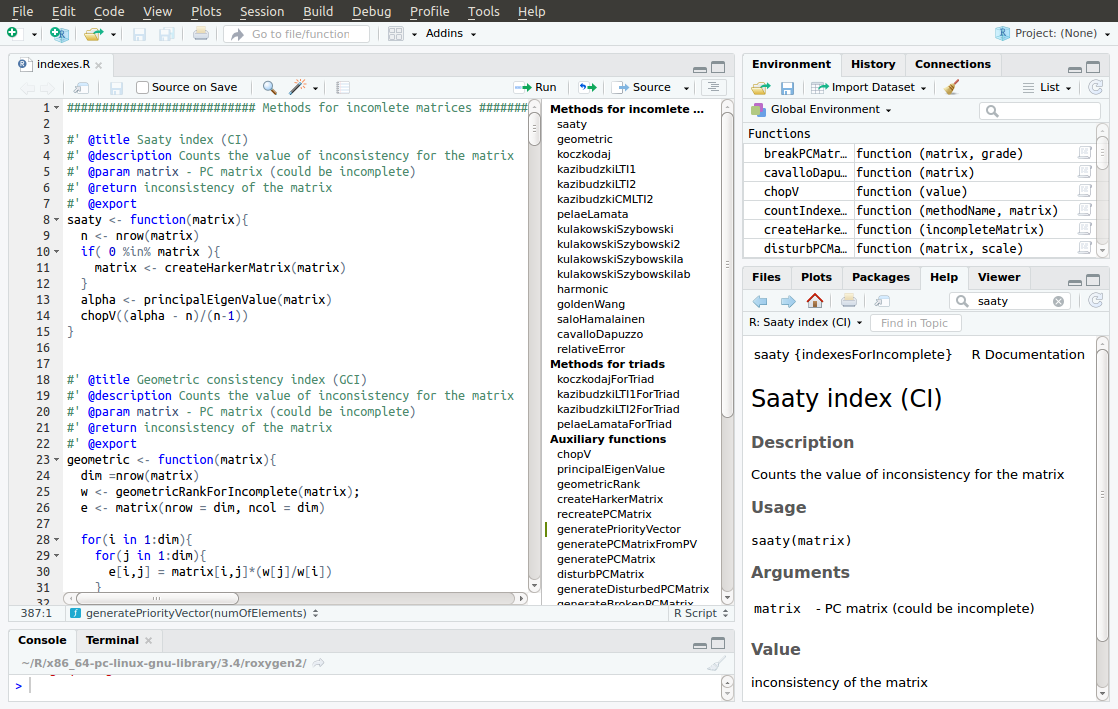
\includegraphics[width=\textwidth]{images/rstudio.png}}
\caption{Program \textit{RStudio}}
\label{fig:rstudio}
\end{figure}


\subsection{Implementation of tests of inconsistency indexes}
Implementation of tests inconsistency indexes consists of two steps:
\begin{enumerate}
  \item Implementation of functions which calculates inconsistency indexes for given matrix (full or incomplete).
  \item Implementation of tests which studies indexes for different matrixes and collects all results of these tests. 
\end{enumerate}

\subsubsection{Implementation of inconsistency indexes}
Sixteen functions which calculate inconsistency indexes using methods described in chapter 3. The functions have been wroten in such a way that allows handle both full and incomplete matrixes. One have not taken account of wrong matrixes, it means nonreciprocal or inconsistent PC matrixes. Each of these function has only one parameter - \textif{PC matrix}. Exceptions are two methods implementing Kulakowski and Szybowski index which additionally take parameters $\alpha, \beta$. The result of each function is value of inconsistency index. The functions have been extended by comments which informs about name of index related to given function, parameters and returned value. It allows to easily read and modify the code. Several examples of functions are presented below.

\begin{figure}[h]
\centerline{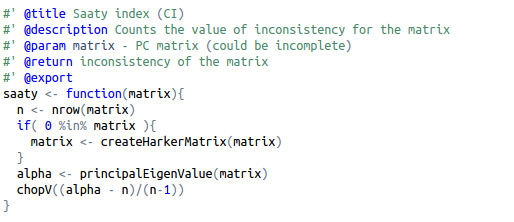
\includegraphics[scale=0.75]{images/kod1.png}}
\caption{The implementation of \textit{Saaty} index}
\label{fig:rstudio}
\end{figure}

\begin{figure}[h]
\centerline{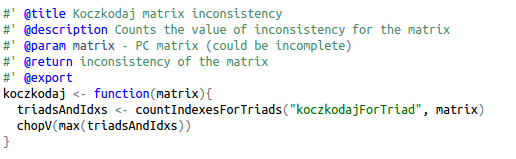
\includegraphics[scale=0.75]{images/kod2.png}}
\caption{The implementation of \textit{Koczkodaj} index}
\label{fig:rstudio}
\end{figure}

\begin{figure}[h]
\centerline{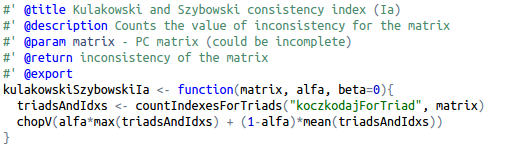
\includegraphics[scale=0.75]{images/kod3.png}}
\caption{The implementation of \textit{Kulakowski and Szybowski} index}
\label{fig:rstudio}
\end{figure}

\begin{figure}[h]
\centerline{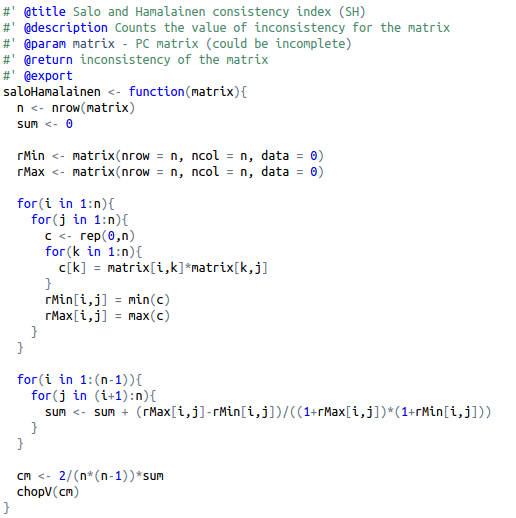
\includegraphics[scale=0.75]{images/kod4.png}}
\caption{The implementation of \textit{Salo and Hamalainen} index}
\label{fig:rstudio}
\end{figure}
It is worth drawing attention to function which is called within the functions intended for indexes based on triads. This function generates triads from a matrix and next returns inconsistency for each o them. However, the way to calculate inconsistency for one triad depends on first function parameter. It informs about function name that calculates inconsistency of a triad specified method.

\begin{figure}[h]
\centerline{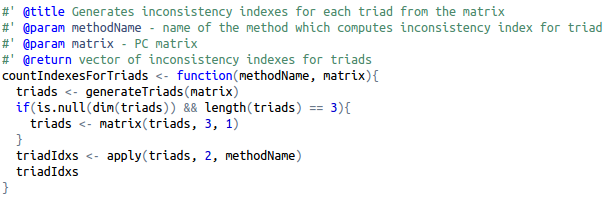
\includegraphics[scale=0.75]{images/kod5.png}}
\caption{The implementation of method \textit{countIndexesForTriads}, which calculates inconsistency for each triad of a specified matrix}
\label{fig:rstudio}
\end{figure}


\subsubsection{Implementation of tests}
In the second step functions, which calculate the quality of the indexes for incomplete matrices, have been created. Functions, which generate specified matrixes, plays an important role. PC matrixes are created depending on size, the level of inconsistency and the degree of incompleteness.

\begin{figure}[h]
\centerline{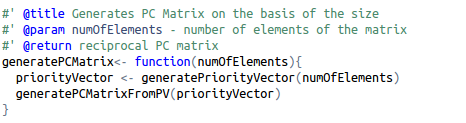
\includegraphics[scale=0.75]{images/kod11.png}}
\caption{The implementation of function \textit{generatePCMatrix} which generates the PC matrix depending on matrix size}
\label{fig:rstudio}
\end{figure}

\begin{figure}[h]
\centerline{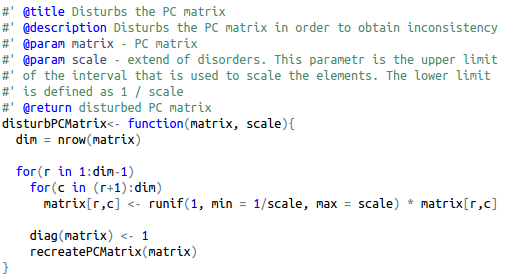
\includegraphics[scale=0.75]{images/kod12.png}}
\caption{The implementation of function \textit{disturbPCMatrix} which disturbs the PC matrix regarding inconsistency depending on given level of inconsistency}
\label{fig:rstudio}
\end{figure}

\begin{figure}[h]
\centerline{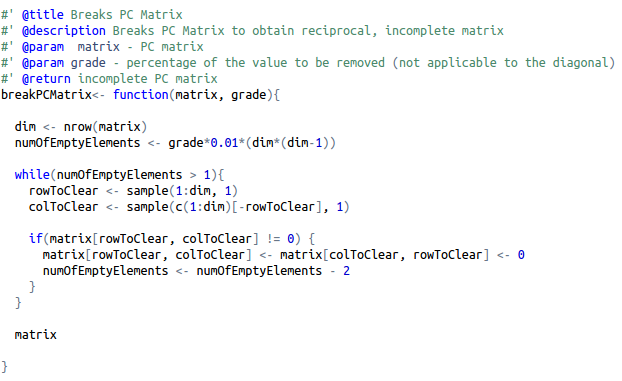
\includegraphics[scale=0.73]{images/kod13.png}}
\caption{The implementation of function \textit{breakPCMatrix} which breaks up the PC matrix regarding incompleteness depending on given degree of incompleteness}
\label{fig:rstudio}
\end{figure}

The last part of functions relates testing how big relative error occurs for inconsistency indexes after deleting some values. To begin with functions, which test one index. They consider matrix size, the level of inconsistency, the degree of incompleteness and the number of attempts which are performed for given matrix.

\begin{figure}[h]
\centerline{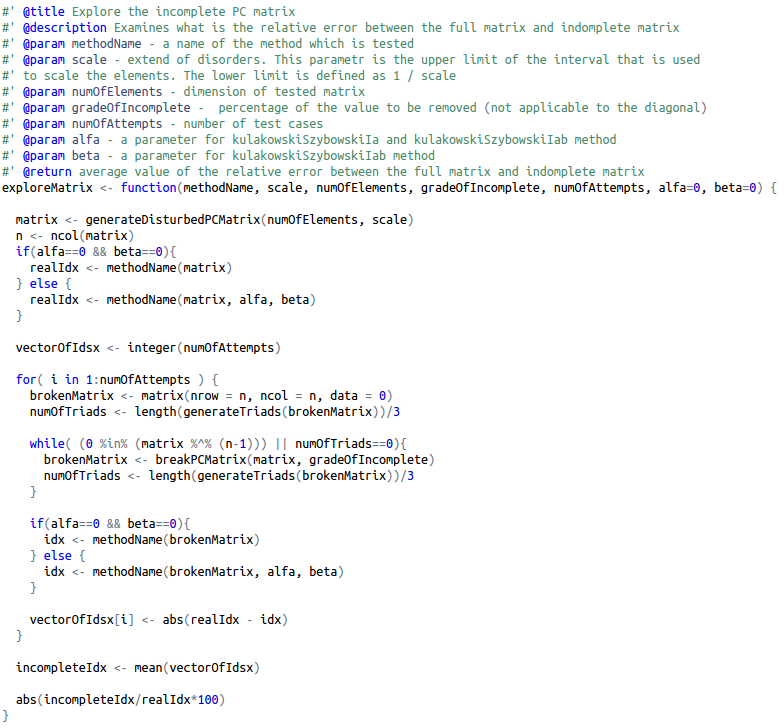
\includegraphics[scale=0.58]{images/kod21.png}}
\caption{The implementation of function \textit{exploreMatrix} which tests given inconsistency index}
\label{fig:rstudio}
\end{figure}

Then functions, which perform tests for each indexes, has been developed basing on the same matrixes. In that the set of matrixes , on which indexes go, is common. Thus, results are reliable and each index is considered the same way.

\begin{figure}[h]
\centerline{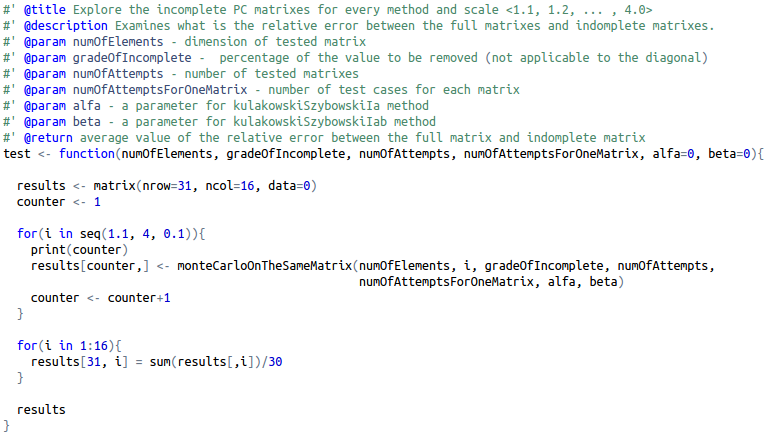
\includegraphics[scale=0.58]{images/kod22.png}}
\caption{The implementation of function \textit{test} which tests all indexes regarding given matrix size and the degree of incompleteness}
\label{fig:rstudio}
\end{figure}


\subsection{Documentation}
Comments in code have been used to generating documentation. the package \textit{roxygen2} has been made for this purpose. It has allowed to easy review code and know the functions./
Exemplary portions of the documentation are presented below.

\begin{figure}[h]
\centerline{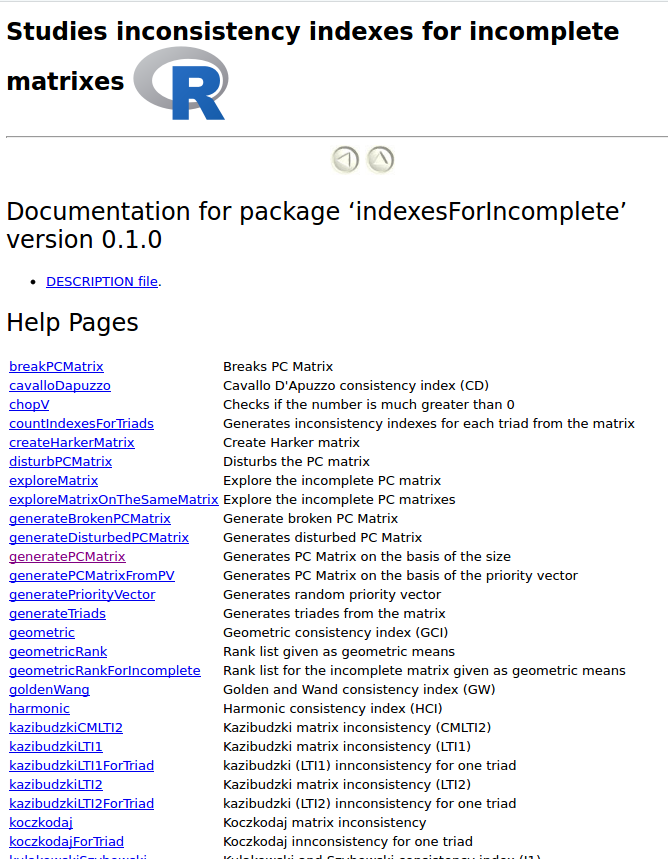
\includegraphics[scale=0.58]{images/kod31.png}}
\caption{The portion of the documentation: general view}
\label{fig:rstudio}
\end{figure}

\begin{figure}[h]
\centerline{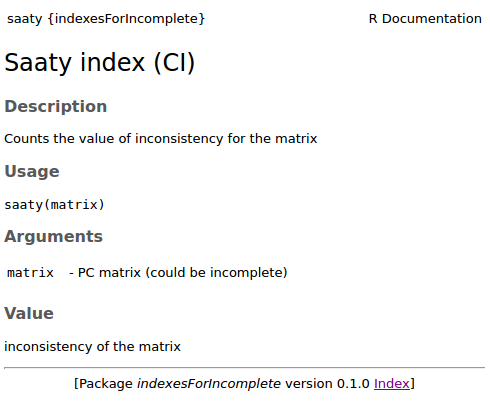
\includegraphics[scale=0.58]{images/kod32.png}}
\caption{The portion of the documentation: function \textit{saaty}}
\label{fig:rstudio}
\end{figure}

\begin{figure}[h]
\centerline{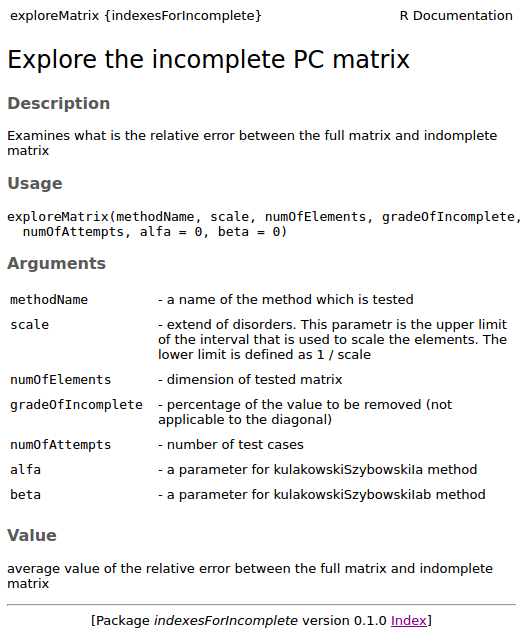
\includegraphics[scale=0.58]{images/kod33.png}}
\caption{The portion of the documentation: function \textit{exploreMatrix}}
\label{fig:rstudio}
\end{figure}
\chapter{Results and discussion}
\label{sec:results}
\section{Results}
The tests were performed using Operating System \textit{Ubuntu 16.04 LTS} and IDE \textit{RStudio}. The results are presented int the following section.

\subsection{Tests taking into account different matrix sizes}
\begin{table}[h]
\begin{center}
\caption{Relative error of inconsistency indexes for incomplete matrices with constant degrees of incompleteness $g=15\%$ and variable matrix size.}
\label{tab:results1}
\begin{tabular}{|c||l|l|l|l|l|c||c|}
\hline Index & n = 4 & n = 7 & n = 8 & n = 10 & n = 15 & mean & rank \\ \hline \hline
saaty & 33,41 & 19,82 & 18,78 & 19,16 & 17,37 & 21,71 & 10 \\ \hline
geometric & 616,68 & 124,73 & 77,94 & 68,62 & 39,13 & 185,42 & 13 \\ \hline
koczkodaj & \textbf{13,86} & \textbf{3,69} & \textbf{2,14} & \textbf{1,62} & \textbf{0,80} & \textbf{4,42} & \textbf{1} \\ \hline
kazibudzkiLTI1 & 24,80 & 10,21 & 6,62 & 4,97 & 2,73 & 9,87 & 6 \\ \hline
kazibudzkiLTI2 & 42,31 & 17,93 & 11,88 & 9,03 & 5,03 & 17,24 & 8 \\ \hline
kazibudzkiCMLTI2 & 35,40 & 17,07 & 13,26 & 11,20 & 6,81 & 16,75 & 7 \\ \hline
pelaeLamata & 44,65 & 19,90 & 13,46 & 10,36 & 5,84 & 18,84 & 9 \\ \hline
kulakSzyb & 20,34 & 7,68 & 4,88 & 3,63 & 1,96 & 7,70 & 5 \\ \hline
kulakSzyb2 & 44,61 & 26,05 & 27,12 & 29,64 & 28,46 & 31,18 & 11 \\ \hline
kulakSzybIa & 16,47 & 5,18 & 3,09 & 2,27 & 1,16 & 5,63 & 3 \\ \hline
kulakSzybIab & 17,40 & 4,89 & 2,81 & 2,04 & 1,01 & 5,63 & 2 \\ \hline
harmonic & 9 573,02 & 1 577,49 & 1 127,33 & 1 066,35 & 866,00 & 2 842,04 & 15 \\ \hline
goldenWang & 115,92 & 54,37 & 43,90 & 43,16 & 36,26 & 58,72 & 12 \\ \hline
saloHamalainen & 381,57 & 205,06 & 176,11 & 160,06 & 136,55 & 211,87 & 14 \\ \hline
cavalloD`Apuzzo & 16,94 & 6,85 & 4,46 & 3,36 & 1,87 & 6,70 & 4 \\ \hline
relativeError & 1 792,64 & 226 313,60 & 746,21 & 100,87 & 20,42 & 45 794,75 & 16 \\ \hline
\end{tabular}
\end{center}
\end{table}

\subsection{Tests taking into account different degrees of incompleteness}
\begin{table}[h]
\begin{center}
\caption{Relative error of inconsistency indexes for incomplete matrices with varying degrees of incompleteness and constant matrix size $n=8$.}
\label{tab:results1}
\begin{tabular}{|c||l|l|l|l|l|c||c|}
\hline Index & $g=4\%$ & $g=7\%$ & $g=14\%$ & $g=25\%$ & $g=50\%$ & mean & rank \\ \hline \hline
saaty & 4,71 & 9,40 & 18,78 & 32,89 & 65,56 & 26,27 & 10 \\ \hline
geometric & 23,60 & 48,44 & 86,61 & 135,68 & 207,99 & 100,46  & 13 \\ \hline
koczkodaj & \textbf{0,48} & \textbf{0,99} & \textbf{2,17} & \textbf{4,52} & 16,41 & 4,92 & 2 \\ \hline
kazibudzkiLTI1 & 2,90 & 4,31 & 6,64 & 10,05 & 23,09 & 9,40 & 6 \\ \hline
kazibudzkiLTI2 & 5,12 & 7,71 & 11,91 & 18,08 & 40,77 & 16,72 & 7 \\ \hline
kazibudzkiCMLTI2 & 5,16 & 8,05 & 13,34 & 22,03 & 61,16 & 21,95 & 9 \\ \hline
pelaeLamata & 5,73 & 8,72 & 13,52 & 20,54 & 45,64 & 18,83 & 8 \\ \hline
kulakSzyb & 2,17 & 3,18 & 4,91 & 7,43 & 17,30 & 7,00 & 5 \\ \hline
kulakSzyb2 & 5,90 & 12,22 & 27,12 & 56,71 & 202,27 & 60,84 & 12 \\ \hline
kulakSzybIa & 1,20 & 1,88 & 3,12 & 5,13 & 13,97 & 5,06 & 3 \\ \hline
kulakSzybIab & 1,00 & 1,65 & 2,84 & 4,74 & \textbf{12,97} & \textbf{4,64} & \textbf{1} \\ \hline
harmonic & 291,74 & 544,60 & 1 152,26 & 1 962,25 & 3 995,58 & 1 589,29 & 16 \\ \hline
goldenWang & 14,23 & 25,23 & 46,18 & 68,83 & 98,24 & 50,54 & 11 \\ \hline
saloHamalainen & 88,40 & 137,70 & 180,17 & 182,54 & 148,74 & 147,51 & 14 \\ \hline
cavalloD`Apuzzo & 1,95 & 2,91 & 4,46 & 6,81 & 16,11 & 6,45 & 4 \\ \hline
relativeError & 18,99 & 20,81 & 206,74 & 68,98 & 1 056,96 & 274,50 & 15 \\ \hline
\end{tabular}
\end{center}
\end{table}

\subsection{Tests taking into account different levels of inconsistency}
Among the tested inconsistency indexes ones, which are given the best results, are presented below. The detailed results are placed in Appendix.
\begin{table}[h]
\begin{center}
\caption{Relative error of inconsistency indexes for incomplete matrices with varying degrees of inconsistency, constant matrix size $n=8$ and constant level of incompleteness $g=15\%$.}
\label{tab:results1}
\begin{tabular}{|c||c|c|c|c|c|c|}
\hline $d$ & koczkodaj & kazibudzkiLTI1 & kulakSzyb & kulakSzybIa & kulakSzybIab & cavalloD`Apuzzo  \\ \hline \hline
1.1 & 4.09 & 6.38 & 6.13 & 4.52 & 4.35 & \textbf{0.49} \\ \hline
1.2 & 3.68 & 6.45 & 5.98 & 4.26 & 4.06 & \textbf{0.96} \\ \hline
1.3 & 3.58 & 6.55 & 5.87 & 4.16 & 3.96 & \textbf{1.37} \\ \hline
1.4 & 3.55 & 6.62 & 5.77 & 4.12 & 3.91 & \textbf{1.80} \\ \hline
1.5 & 3.19 & 6.35 & 5.42 & 3.80 & 3.59 & \textbf{2.02} \\ \hline
1.6 & 3.26 & 6.57 & 5.46 & 3.84 & 3.64 & \textbf{2.39} \\ \hline
1.7 & 3.03 & 6.59 & 5.35 & 3.71 & 3.48 & \textbf{2.81} \\ \hline
1.8 & \textbf{2.47} & 6.45 & 5.13 & 3.31 & 3.04 & 3.07 \\ \hline
1.9 & \textbf{2.47} & 6.65 & 5.26 & 3.35 & 3.06 & 3.34 \\ \hline
2.0 & \textbf{2.20} & 6.66 & 5.13 & 3.16 & 2.85 & 3.64 \\ \hline
2.1 & \textbf{2.38} & 6.51 & 4.93 & 3.21 & 2.93 & 3.83 \\ \hline
2.2 & \textbf{2.16} & 6.52 & 4.81 & 3.04 & 2.76 & 4.09 \\ \hline
2.3 & \textbf{2.14} & 6.66 & 4.89 & 3.07 & 2.80 & 4.25 \\ \hline
2.4 & \textbf{2.00} & 6.67 & 4.85 & 2.98 & 2.67 & 4.49 \\ \hline
2.5 & \textbf{1.96} & 6.59 & 4.73 & 2.91 & 2.63 & 4.71 \\ \hline
2.6 & \textbf{1.73} & 6.62 & 4.72 & 2.81 & 2.48 & 4.87 \\ \hline
2.7 & \textbf{1.94} & 6.79 & 4.73 & 2.96 & 2.67 & 5.14 \\ \hline
2.8 & \textbf{1.75} & 6.67 & 4.64 & 2.78 & 2.47 & 5.24 \\ \hline
2.9 & \textbf{1.56} & 6.67 & 4.54 & 2.68 & 2.38 & 5.60 \\ \hline
3.0 & \textbf{1.82} & 6.71 & 4.68 & 2.84 & 2.51 & 5.56 \\ \hline
3.1 & \textbf{1.47} & 6.69 & 4.48 & 2.62 & 2.30 & 5.74 \\ \hline
3.2 & \textbf{1.46} & 6.52 & 4.40 & 2.59 & 2.28 & 5.75 \\ \hline
3.3 & \textbf{1.48} & 6.85 & 4.57 & 2.65 & 2.35 & 6.14 \\ \hline
3.4 & \textbf{1.38} & 6.60 & 4.30 & 2.53 & 2.23 & 6.15 \\ \hline
3.5 & \textbf{1.17} & 6.60 & 4.25 & 2.40 & 2.10 & 6.50 \\ \hline
3.6 & \textbf{1.25} & 6.73 & 4.39 & 2.50 & 2.18 & 6.65 \\ \hline
3.7 & \textbf{1.18} & 6.83 & 4.41 & 2.48 & 2.19 & 6.77 \\ \hline
3.8 & \textbf{1.24} & 6.59 & 4.17 & 2.40 & 2.09 & 6.68 \\ \hline
3.9 & \textbf{1.28} & 6.73 & 4.25 & 2.47 & 2.19 & 6.79 \\ \hline
4.0 & \textbf{1.11} & 6.52 & 4.17 & 2.35 & 2.06 & 6.79 \\ \hline \hline
mean & \textbf{2.13} & 6.61 & 4.88 & 3.08 & 2.81 & 4.45 \\ \hline 
\end{tabular}
\end{center}
\end{table}



\section{Discussion}
Analyzing the above results, one can draw several conclusions.

\subsection{Tests taking into account different matrix sizes}
Along with growth of the matrix size, examined relative error decreases. Considering the best indexes, the relative error is between $13$ and $17$ percent for small matrices (size $4$) so it is relatively big. However, it decreases rapidly, when the size of PC matrix increases. For matrix of size $7$ indexes exist which give the results in range $3 - 5 \%$, what is a acceptable score. For PC matrices with a significant size (over $10$ concepts), the relative error is just about $1 - 2 \%$, what is an really good score.

Definitely, the best index found was out \textit{Koczkodaj index}. It wins in each test regardless of the matrix size. It gives really satisfying results for of size $7$ and more matrices. Good results were obtained also through indexes \textit{kulakowskiSzybowskiIab}, \textit{kulakowskiSzybowskiIa} and \textit{cavalloD`Apuzzo}. It seems that these indexes are reliable. Absolutely one should reject indexes \textit{relativeError}, \textit{harmonic}, \textit{saloHamalainen}, \textit{geometric}, \textit{goldenWang} for incomplete matrices. Results obtained through these methods show that score for examined inconsistency for incomplete matrices can differ significantly from a right values.

It is worth noticing that the presented results involve matrices with the degree of incompleteness equal to $15\%$. It means that $7$ comparisons are missing for matrices with size $n = 10$. The results will be different from presented in table 5.1. for other degrees of incompleteness. Impact on the degree of incompleteness on tested relative error is shown consecutive experiments.

\subsection{Tests taking into account different degrees of incompleteness}
Along with growth of the degree of incompleteness, examined relative error grows. Considering the best indexes, the relative error amount to just about $1 - 2\%$ percent for degree of incompleteness (size $4$) so it is really satisfying. However, it increases slowly, when the degree of incompleteness decreases. For the degree of incompleteness $g=14\%$ exist indexes which give the results about $2 - 3 \%$, what is a gratifying score. The relative error is equal about a dozen percent for significant matrices ($g=50\%$).

Definitely, the best indexes came out \textit{Koczkodaj index} and \textit{kulakowskiSzybowskiIab}. First one wins in most cases and gives really satisfy the results. Second one improves along with the growth of the degree of incompleteness. It obtained a significant advantage over other methods in the last test, what caused that the average value turned out to be the lowest. 
The good results were obtained also through indexes \textit{kulakowskiSzybowskiIa} and \textit{cavalloD`Apuzzo}. It seems that these indexes are reliable. Absolutely one should reject indexes \textit{harmonic}, \textit{relativeError}, \textit{saloHamalainen}, \textit{geometric}. Results obtained through these methods shows that score examined inconsistency for incomplete matrices can differ significantly from the right values.

It is worth noticing that the presented results involve matrices with the size $8\%$. The results will be different from presented in table 5.2. for other matrix sizes. Impact on the degree of incompleteness on tested relative error was shown in previous experiments.

\subsection{Tests taking into account different levels of inconsistency}
All tests for different matrix sizes and degrees of incompleteness was performed taking into account varying levels of inconsistency. The scale of this incompleteness is proportional to the value $d$ included in table 5.3. This table shows detailed results for which average values were presented in table 5.1. It is worth taking a closer look at these scores. They point out that the quality of inconsistency indexes is determined also by the level of inconsistency.

The lowest values of the relative error was obtained by \textit{Koczkodaj index}, what was discussed before. One should notice and emphasize that it gives the best results only from particular moment in which the level of inconsistency in matrix begins to grow. For small inconsistencies, the most satisfying index is \textit{Cavallo and D`Apuzzo index}. This in interesting regularity which indicates that the choice of inconsistency index for incomplete matrices should depend on the level of inconsistency. 

It is worth noticing that this regularity repeats in each of the performed tests. For small level of inconsistency, regardless of the matrix size and the degree od incompleteness, \textit{Cavallo and D`Apuzzo index} comes out to be the best. The results presented in Appendix confirm it.

\subsection{General discussion}
Certainly, the tests managed to show that the error increases with a growth of the level of incompleteness. At the same time, it decreases when the size of the matrix increases. However, the most important question was about which indexes cope well with incomplete matrices. The Koczkodaj index ([sub:Koczkodaj-index]) won in 9 out of 10 tests and its average error in both cases turns out to be the lowest (below $5\%$). The next places are occupied by two indexes introduced by Kułakowski and Szybowski ([eq:Ia], [eq:Iab]) and Cavallo and D'Apuzzo index ([sub:Cavallo-and-D’Apuzzo]). It is worth noting that all of these indexes are based on triads.

A question about what makes the Koczkodaj index giving such good results and whether is it worth using, may arise. One should return to the definition of this index ([eq:K]) and notice that it is equal to the value of the most inconsistency triad. Therefore, if the level of incompleteness is low, there is a good chance that after deletion of some values from the matrix and recalculation at the index the value of it will not change at all. It will only change if the element included in the most inconsistent triad is removed. However, in many cases, the examination of the full matrix and th matrix after removing some values give exactly the same results (the error is $0\%$). This is the only index of this kind among those presented in the paper.

If one uses the Koczkodaj index, one may be worried that the removed comparison belonged to the most inconsistent triad. In such a case, it is difficult to predict what error will be contained in the index of the incomplete matrix. It seems that one should pay particular attention to the indexes proposed by Kułakowski and Szybowski. First of them ([eq:I1]) averages the inconsistencies of the triads. Therefore, it is safe and gives good results (in both tests it took the sixth place and achieved an error below $8\%$). From this perspective, another index suggested by the same authors ([eq:Ia]) turns out to be very interesting. In the tests it took the third place. It has the parameter $\alpha$ allowing to determine the effect of the greatest inconsistency of the triad $\left(\alpha\right)$ and the average $\left(1-\alpha\right)$. In the tests carried out, the parameter $\alpha$ was $0.4$.
\chapter{Summary}
\label{sec:summary}

\printbibliography

\chapter{Appendix}

The detailed results of the inconsistency indexes tests are presented in this section. Each description of the table includes the information about the degree of incompleteness ($g$) and the matrix size ($n$). The results are ordered by the value $d$ which define the level of inconsistency (see~5.2.3 on page~32).





%n=4. g=15
\newpage
\textbf{Table 7.1.} Relative error of the inconsistency indexes for incomplete matrices ($g=15\%$, $n=4$)
\begin{adjustbox}{angle=90}
  \setstretch{1.167}
  \begin{center}
    \small{
    \begin{tabular}{|l|llllllllllllllll|}
      \hline $d$&$CI$&$GCI$&$K$&$ML$&$ML*$&$CM*$&$PL$&$I_1$&$I_2$&$I_{\alpha}$&$I_{\alpha.\beta}$&$HCI$&$GW$&$CM$&$I_{CD}$&$RE$\\ \hline \hline
1.1&33.19&12104.96&17.50&24.29&40.80&40.59&40.82&23.73&47.53&20.25&21.48&176471.17&924.12&2591.56&1.68&97.42  \\ 
1.2&33.52&1567.67&18.85&25.93&45.06&44.05&45.18&24.47&46.35&21.30&22.53&32823.18&359.14&1063.09&3.89&308.02  \\ 
1.3&33.31&725.44&17.41&24.95&43.15&41.54&43.35&23.15&46.27&19.89&20.99&12787.44&213.47&744.18&5.02&71.52  \\ 
1.4&33.21&645.42&16.20&23.81&40.22&37.90&40.50&22.10&45.79&18.66&19.61&16629.05&204.06&623.89&5.95&45.49  \\ 
1.5&33.08&353.33&15.83&24.97&41.91&38.20&42.44&22.53&46.35&18.63&19.59&5285.36&126.31&482.26&8.31&68.22  \\ 
1.6&33.12&326.60&15.89&25.01&42.02&37.85&42.63&22.18&46.25&18.53&19.50&4959.79&115.14&492.77&8.97&46.59  \\ 
1.7&33.39&209.28&16.05&25.78&44.03&38.61&44.95&22.35&45.54&18.66&19.60&2795.70&101.82&377.33&10.91&52.22  \\ 
1.8&33.59&141.17&14.74&24.06&41.89&35.46&43.09&20.39&44.07&17.02&17.88&1907.41&77.62&283.58&12.05&102.17  \\ 
1.9&33.09&345.42&15.18&24.71&42.12&36.38&43.18&21.25&45.07&17.67&18.76&3620.01&103.23&397.19&11.62&245.15  \\ 
2&33.56&154.50&13.95&23.92&41.22&34.33&42.78&19.98&44.31&16.37&17.34&1695.00&62.10&256.96&13.63&20761.78  \\ 
2.1&33.54&151.87&14.90&26.15&43.94&36.30&45.70&22.00&45.23&17.72&18.39&2641.03&84.38&292.25&15.32&89.12  \\ 
2.2&33.54&128.82&14.04&24.74&41.61&34.29&43.22&20.30&45.29&16.60&17.66&2376.14&76.89&266.18&15.08&422.96  \\ 
2.3&33.30&95.04&14.16&24.85&42.44&35.36&44.18&20.23&44.78&16.64&17.78&1634.53&68.92&229.25&15.88&101.10  \\ 
2.4&33.57&211.08&13.77&24.51&42.04&34.03&43.94&19.66&44.55&16.14&17.13&1658.24&76.01&279.75&16.24&81.57  \\ 
2.5&33.84&90.66&14.34&26.48&45.19&36.25&47.81&21.17&44.31&16.99&17.56&1421.62&67.20&208.67&19.02&164.15  \\ 
2.6&33.42&81.83&13.50&25.29&43.13&34.46&45.72&19.90&44.36&16.01&16.80&1573.20&68.03&214.57&19.25&69.40  \\ 
2.7&33.05&109.41&13.05&24.51&41.66&34.11&44.08&19.87&44.36&15.76&16.76&992.45&58.29&239.06&18.82&1743.72  \\ 
2.8&33.27&166.17&12.98&24.78&42.11&33.69&44.91&19.82&44.04&15.67&16.60&1445.28&61.24&244.57&19.75&72.94  \\ 
2.9&33.21&160.23&12.01&24.05&40.72&32.46&43.71&18.99&44.09&14.73&15.68&3339.37&67.32&208.39&20.82&2333.47  \\ 
3&33.24&85.97&12.12&24.47&41.06&32.71&44.14&19.24&44.41&14.96&15.89&1250.55&57.19&195.25&21.98&332.82  \\ 
3.1&33.45&56.19&12.98&25.66&43.99&34.58&47.42&19.47&43.82&15.56&16.52&798.47&50.10&177.58&23.02&69.28  \\ 
3.2&33.32&62.35&12.88&25.19&43.30&34.40&46.43&19.84&43.68&15.58&16.15&1035.09&52.63&192.25&21.30&2688.16  \\ 
3.3&33.87&69.95&11.43&23.98&40.86&32.59&44.75&18.20&43.45&14.09&15.02&898.67&47.98&168.69&23.84&96.62  \\ 
3.4&33.91&64.68&12.07&23.78&41.53&32.61&45.21&18.29&42.94&14.44&15.17&998.13&50.90&182.56&21.56&54.37  \\ 
3.5&33.55&65.82&12.88&26.69&45.71&35.43&50.14&19.25&43.77&15.40&16.32&830.19&48.11&149.19&27.25&99.53  \\ 
3.6&33.55&53.38&11.45&24.17&41.34&32.62&45.62&18.09&43.33&14.05&15.06&765.32&42.11&159.29&25.92&406.00  \\ 
3.7&33.53&55.87&12.13&24.93&42.65&34.01&46.70&18.49&44.12&14.60&15.50&1116.55&48.22&193.19&24.59&57.03  \\ 
3.8&33.48&71.37&11.52&25.63&43.51&34.16&48.50&20.03&43.33&14.85&15.31&1303.35&59.66&167.63&27.58&40.68  \\ 
3.9&33.30&96.37&12.26&25.20&42.90&34.07&46.90&19.45&44.01&15.04&15.92&1453.40&66.04&214.01&24.72&368.10  \\ 
4&33.21&49.52&9.71&21.61&37.22&28.93&41.43&15.81&42.82&12.13&13.51&684.82&39.42&151.90&24.37&22689.73  \\ \hline \hline
Mean&33.41&616.68&13.86&24.80&42.31&35.40&44.65&20.34&44.61&16.47&17.40&9573.02&115.92&381.57&16.94&1792.64  \\ \hline
\end{tabular}
}
\end{center}
\end{adjustbox}




%n=6. g=15
\newpage
\textbf{Table 7.2.} Relative error of the inconsistency indexes for incomplete matrices ($g=15\%$, $n=6$)
\begin{adjustbox}{angle=90}
  \setstretch{1.03}
  \begin{center}
    \begin{tabular}{|l|llllllllllllllll|}
      \hline $d$ &
$CI$&$GCI$&$K$&$ML$&$ML*$&$CM*$&$PL$&$I_1$&$I_2$&$I_{\alpha}$&$I_{\alpha.\beta}$&$HCI$&$GW$&$CM$&$I_{CD}$&$RE$\\ \hline \hline
1.1&20.10&1868.93&6.43&10.31&17.89&17.64&17.91&9.94&26.51&7.46&7.29&24720.24&470.82&1378.25&0.78&42.04  \\ 
1.2&19.80&626.24&5.76&10.17&17.52&16.63&17.59&9.51&26.48&7.04&6.82&7130.13&228.74&695.06&1.47&31.32  \\ 
1.3&19.91&315.86&5.84&10.01&17.24&15.71&17.39&9.10&26.38&6.84&6.64&3767.46&143.24&463.31&2.09&345.58  \\ 
1.4&19.77&121.52&5.38&10.12&18.08&15.77&18.36&8.82&26.37&6.53&6.39&1705.04&80.19&327.93&2.77&27.44  \\ 
1.5&20.23&123.06&5.45&10.10&17.46&15.24&17.82&8.73&25.94&6.48&6.26&1329.51&62.25&269.96&3.23&6787322  \\ 
1.6&19.96&69.34&4.85&10.29&17.74&15.30&18.21&8.69&26.16&6.15&5.91&1011.94&55.21&234.21&3.87&26.59  \\ 
1.7&19.65&56.03&4.29&9.65&16.82&14.58&17.36&8.01&26.04&5.60&5.35&907.14&51.93&224.46&3.99&43.59  \\ 
1.8&20.06&39.81&4.78&10.60&18.60&15.90&19.37&8.55&26.04&6.07&5.79&735.89&45.47&185.14&4.72&20.31  \\ 
1.9&20.23&34.56&4.18&10.35&18.09&15.58&19.01&8.16&25.94&5.56&5.24&581.36&36.39&159.97&5.26&16.97  \\ 
2&19.76&36.44&3.99&10.13&17.84&15.35&18.87&7.91&26.04&5.39&5.11&526.35&35.92&158.19&5.44&17.64  \\ 
2.1&19.73&37.17&4.04&10.20&17.99&15.90&19.24&7.86&26.10&5.40&5.12&408.66&30.08&150.79&5.84&31.73  \\ 
2.2&19.96&36.53&3.89&10.43&18.45&15.97&19.84&7.86&25.98&5.35&5.04&398.67&30.98&148.00&6.31&34.77  \\ 
2.3&19.93&23.78&3.53&10.24&17.86&16.25&19.40&7.70&25.98&5.05&4.73&332.65&26.02&131.13&6.66&23.92  \\ 
2.4&19.97&30.74&3.41&10.30&17.85&16.16&19.56&7.69&25.96&5.00&4.68&302.98&22.19&126.65&7.01&559.80  \\ 
2.5&19.75&24.94&3.64&10.31&18.15&17.09&20.00&7.53&26.05&5.06&4.76&286.94&23.32&115.85&7.26&26.15  \\ 
2.6&19.73&26.64&3.52&10.17&18.08&17.72&20.21&7.41&25.91&4.93&4.62&307.05&26.22&121.68&7.28&16.48  \\ 
2.7&19.77&21.14&3.25&9.94&17.34&17.36&19.53&7.20&26.05&4.71&4.41&250.59&21.04&100.36&7.64&39.40  \\ 
2.8&19.97&21.97&3.11&10.14&18.02&16.96&20.42&7.18&25.90&4.72&4.40&252.98&20.64&103.64&8.17&21.85  \\ 
2.9&19.55&20.94&2.83&10.10&17.69&17.09&20.07&7.15&26.04&4.52&4.19&261.89&20.84&103.84&8.22&21.15  \\ 
3&19.89&19.99&3.03&10.48&18.12&18.07&20.87&7.33&25.87&4.72&4.35&217.32&20.21&99.81&9.08&27.14  \\ 
3.1&19.75&19.73&2.86&10.03&17.80&18.23&20.81&6.85&25.86&4.42&4.09&207.25&19.56&89.76&9.07&32.38  \\ 
3.2&19.70&18.36&2.89&10.47&18.70&18.83&22.01&7.03&25.98&4.55&4.25&214.99&19.02&86.30&9.41&15.74  \\ 
3.3&19.75&20.36&2.69&10.46&18.50&17.92&21.52&7.08&26.01&4.48&4.17&220.45&19.47&97.12&9.43&17.05  \\ 
3.4&19.55&19.49&2.26&10.33&18.02&17.37&21.12&7.01&25.98&4.22&3.88&195.49&18.51&89.56&9.64&27.51  \\ 
3.5&19.73&19.08&2.23&10.21&17.63&18.12&20.78&6.86&26.00&4.16&3.81&192.48&19.15&82.64&9.96&130.74  \\ 
3.6&19.83&16.85&2.66&10.33&18.37&18.30&22.08&6.77&25.93&4.31&3.99&174.28&16.35&77.63&10.06&178.79  \\ 
3.7&19.58&19.05&2.27&9.83&17.47&17.62&21.04&6.44&26.01&3.97&3.69&186.37&17.67&84.63&9.91&254.39  \\ 
3.8&19.76&18.52&2.86&10.61&18.97&20.55&23.18&6.92&26.04&4.51&4.21&178.71&18.07&83.83&10.49&18.02  \\ 
3.9&19.55&17.26&2.42&10.04&17.76&19.14&21.43&6.56&26.03&4.13&3.82&168.91&17.06&86.59&10.04&24.04  \\ 
4&19.55&17.59&2.37&10.02&17.77&19.90&21.99&6.48&26.06&4.04&3.73&150.92&14.63&75.63&10.43&13.09  \\ \hline \hline
Mean&19.82&124.73&3.69&10.21&17.93&17.07&19.90&7.68&26.05&5.18&4.89&1577.49&54.37&205.06&6.85&226313.60  \\ \hline
\end{tabular}
\end{center}
\end{adjustbox}




%n=8. g=15
\newpage
\textbf{Table 7.3.} Relative error of the inconsistency indexes for incomplete matrices ($g=15\%$, $n=8$)
\begin{adjustbox}{angle=90}
  \setstretch{1.03}
  \begin{center}
    \begin{tabular}{|l|llllllllllllllll|}
      \hline $d$ &
$CI$&$GCI$&$K$&$ML$&$ML*$&$CM*$&$PL$&$I_1$&$I_2$&$I_{\alpha}$&$I_{\alpha.\beta}$&$HCI$&$GW$&$CM$&$I_{CD}$&$RE$\\ \hline \hline
1.1&18.96&1225.95&4.09&6.38&11.35&11.15&11.37&6.13&27.13&4.52&4.36&17996.79&392.32&1182.47&0.49&13.90  \\ 
1.2&18.83&316.10&3.68&6.46&11.44&10.86&11.50&5.99&27.13&4.26&4.06&4579.40&174.75&580.40&0.96&13.93  \\ 
1.3&18.98&180.77&3.58&6.56&11.76&10.75&11.88&5.87&27.06&4.17&3.96&2345.13&113.61&416.96&1.38&36.61  \\ 
1.4&19.05&84.52&3.55&6.62&11.78&10.65&11.97&5.77&27.11&4.12&3.92&1425.06&75.22&303.49&1.80&250.90  \\ 
1.5&19.04&76.86&3.19&6.36&11.33&10.44&11.59&5.42&27.03&3.81&3.60&1043.73&65.41&263.84&2.03&16.10  \\ 
1.6&18.91&45.10&3.27&6.57&11.82&11.15&12.21&5.47&27.12&3.85&3.64&786.59&49.24&218.35&2.40&14.15  \\ 
1.7&18.82&31.42&3.03&6.59&11.78&11.55&12.31&5.35&27.09&3.71&3.49&595.07&38.12&182.82&2.82&27.71  \\ 
1.8&18.92&25.39&2.48&6.45&11.49&11.29&12.07&5.13&27.08&3.31&3.04&490.23&30.36&159.28&3.07&29.66  \\ 
1.9&18.82&24.17&2.47&6.66&11.75&11.65&12.43&5.26&27.13&3.36&3.07&441.43&30.10&147.44&3.35&29.23  \\ 
2 &18.84&20.33&2.20&6.67&11.81&12.27&12.60&5.14&27.13&3.16&2.85&374.75&27.41&130.04&3.65&8708.76  \\ 
2.1&18.91&16.51&2.39&6.52&11.64&12.49&12.57&4.94&27.07&3.21&2.94&306.72&21.69&114.90&3.84&12.41  \\ 
2.2&18.92&15.13&2.17&6.52&11.87&13.02&13.03&4.81&27.04&3.05&2.77&279.28&20.36&106.14&4.10&27.71  \\ 
2.3&18.74&20.59&2.15&6.66&12.04&13.08&13.24&4.90&27.19&3.07&2.80&273.36&21.15&115.29&4.26&1144.60  \\ 
2.4&18.92&17.16&2.01&6.68&11.93&13.20&13.23&4.85&27.04&2.98&2.68&266.67&21.47&110.77&4.49&18.08  \\ 
2.5&18.58&15.50&1.97&6.59&11.84&14.02&13.34&4.74&27.15&2.92&2.63&222.52&17.75&99.31&4.71&10.70  \\ 
2.6&18.74&15.37&1.73&6.63&11.81&13.35&13.33&4.72&27.06&2.81&2.48&233.57&20.21&97.41&4.87&29.43  \\ 
2.7&18.83&14.81&1.95&6.80&12.40&15.19&14.30&4.73&27.11&2.96&2.67&212.86&18.45&94.03&5.15&10.80  \\ 
2.8&18.64&15.54&1.76&6.67&12.06&14.50&14.03&4.64&27.16&2.79&2.48&193.15&16.09&88.45&5.24&200.86  \\ 
2.9&18.64&14.81&1.56&6.67&12.00&14.44&14.07&4.54&27.24&2.68&2.39&166.18&15.05&82.83&5.60&10.76  \\ 
3&18.89&15.89&1.83&6.72&11.83&15.41&13.82&4.68&27.03&2.84&2.52&181.14&15.87&82.41&5.56&11.36  \\ 
3.1&18.81&14.19&1.48&6.69&12.18&14.51&14.51&4.49&27.06&2.62&2.30&175.17&14.97&78.67&5.74&13.32  \\ 
3.2&18.81&17.16&1.47&6.53&11.74&14.16&13.98&4.40&27.03&2.60&2.29&154.99&14.71&78.09&5.76&11651.28  \\ 
3.3&18.54&15.02&1.49&6.85&12.33&15.08&14.87&4.57&27.22&2.66&2.35&158.88&14.60&77.46&6.14&13.70  \\ 
3.4&18.67&14.87&1.38&6.61&12.06&14.50&14.76&4.31&27.12&2.53&2.23&142.38&13.50&72.61&6.16&10.47  \\ 
3.5&18.67&14.36&1.17&6.60&11.90&14.22&14.74&4.26&27.09&2.41&2.10&128.52&11.69&65.40&6.50&15.35  \\ 
3.6&18.61&13.83&1.26&6.74&12.04&15.27&14.91&4.39&27.11&2.50&2.18&136.06&12.42&68.00&6.65&16.50  \\ 
3.7&18.54&14.01&1.18&6.83&12.28&14.44&15.31&4.41&27.26&2.49&2.20&138.96&15.05&70.51&6.77&10.50  \\ 
3.8&18.70&14.00&1.25&6.59&12.04&14.90&15.14&4.18&27.11&2.41&2.10&125.35&11.25&64.67&6.69&11.43  \\ 
3.9&18.56&14.36&1.28&6.73&12.42&15.84&15.87&4.25&27.14&2.48&2.20&120.27&11.68&67.99&6.79&12.50  \\ 
4 & 18.50&14.46&1.12&6.53&11.70&14.57&14.80&4.17&27.24&2.36&2.06&125.58&12.49&63.20&6.79&13.70  \\ \hline \hline
Mean & 18.78&77.94&2.14&6.62&11.88&13.26&13.46&4.88&27.12&3.09&2.81&1127.33&43.90&176.11&4.46&746.21  \\ \hline
\end{tabular}
\end{center}
\end{adjustbox}




%n=10. g=15
\newpage
\textbf{Table 7.4.} Relative error of the inconsistency indexes for incomplete matrices ($g=15\%$, $n=10$)
\begin{adjustbox}{angle=90}
  \setstretch{1.03}
  \begin{center}
    \begin{tabular}{|l|llllllllllllllll|}
      \hline $d$ &
$CI$&$GCI$&$K$&$ML$&$ML*$&$CM*$&$PL$&$I_1$&$I_2$&$I_{\alpha}$&$I_{\alpha.\beta}$&$HCI$&$GW$&$CM$&$I_{CD}$&$RE$\\ \hline \hline
1.1&19.53&1155.16&3.92&4.95&8.90&8.70&8.91&4.75&29.43&3.95&3.88&16874.42&410.53&1099.63&0.37&12.99  \\ 
1.2&19.39&253.54&3.46&4.87&8.86&8.38&8.91&4.50&29.56&3.55&3.45&4528.27&170.36&541.47&0.72&14.48  \\ 
1.3&19.38&120.88&2.95&4.82&8.65&8.08&8.74&4.32&29.59&3.19&3.05&2174.76&107.84&366.14&1.01&23.06  \\ 
1.4&19.49&84.28&2.78&4.88&8.79&8.37&8.95&4.24&29.51&3.08&2.92&1481.84&84.23&300.03&1.29&14.45  \\ 
1.5&19.34&42.46&2.55&4.77&8.56&8.67&8.77&4.04&29.69&2.87&2.71&957.94&58.79&224.77&1.55&13.71  \\ 
1.6&19.29&44.20&2.49&4.94&8.82&9.42&9.12&4.09&29.59&2.83&2.64&727.91&53.04&206.90&1.86&11.50  \\ 
1.7&19.41&28.15&2.38&4.90&8.78&9.85&9.16&3.99&29.59&2.77&2.58&592.50&39.57&176.37&2.03&11.84  \\ 
1.8&19.22&22.33&1.88&4.89&8.81&9.60&9.31&3.86&29.64&2.43&2.20&448.98&30.53&148.97&2.30&11.27  \\ 
1.9&19.30&16.87&1.91&5.03&9.05&10.25&9.63&3.91&29.61&2.46&2.21&395.36&29.29&129.76&2.56&19.11  \\ 
2&19.27&18.50&1.75&4.85&8.82&10.15&9.49&3.69&29.59&2.30&2.07&341.46&24.36&118.92&2.65&14.77  \\ 
2.1&19.19&15.15&1.48&4.93&9.00&10.17&9.77&3.67&29.67&2.17&1.91&303.67&24.69&112.30&2.85&17.30  \\ 
2.2&19.25&14.38&1.71&4.88&8.87&11.27&9.79&3.62&29.65&2.27&2.03&270.64&20.74&101.79&3.03&23.24  \\ 
2.3&19.18&13.76&1.57&5.01&8.96&11.54&9.92&3.68&29.71&2.21&1.96&247.99&18.55&97.39&3.26&10.62  \\ 
2.4&19.07&13.76&1.44&4.92&9.00&11.47&10.13&3.52&29.71&2.11&1.86&229.97&16.87&90.29&3.35&9.43  \\ 
2.5&19.15&12.40&1.47&5.16&9.39&11.90&10.64&3.64&29.68&2.17&1.91&216.72&16.58&84.43&3.65&11.09  \\ 
2.6&19.19&13.72&1.30&5.06&9.11&11.80&10.41&3.56&29.68&2.06&1.78&199.80&15.48&81.51&3.76&11.59  \\ 
2.7&19.03&13.46&1.25&5.05&9.25&12.09&10.77&3.48&29.70&2.01&1.75&188.03&15.59&83.84&3.89&9.17  \\ 
2.8&19.14&12.62&1.15&4.92&8.97&11.46&10.50&3.39&29.64&1.94&1.67&180.37&14.13&79.28&3.93&9.21  \\ 
2.9&19.15&12.95&1.14&5.07&9.20&11.94&10.79&3.45&29.66&1.93&1.65&179.07&14.91&77.85&4.09&8.95  \\ 
3&19.04&12.77&1.08&5.03&9.12&11.98&10.82&3.38&29.66&1.91&1.64&157.43&13.32&72.07&4.25&9.19  \\ 
3.1&19.12&13.47&1.16&5.06&9.29&13.14&11.21&3.38&29.68&1.95&1.69&159.90&13.95&70.73&4.33&2667.27  \\ 
3.2&19.12&13.46&0.92&5.06&9.23&11.96&11.23&3.29&29.66&1.79&1.51&133.49&10.90&62.17&4.59&11.42  \\ 
3.3&18.90&13.40&0.93&5.09&9.20&12.67&11.27&3.32&29.68&1.82&1.55&136.33&12.09&62.06&4.70&9.53  \\ 
3.4&18.97&13.98&0.99&5.02&9.23&12.80&11.44&3.26&29.64&1.83&1.55&136.32&12.20&64.45&4.64&8.68  \\ 
3.5&19.02&13.45&0.85&5.04&9.22&12.30&11.58&3.23&29.65&1.77&1.50&131.77&12.14&62.60&4.82&11.26  \\ 
3.6&18.89&13.71&0.89&5.00&9.09&13.36&11.58&3.20&29.70&1.77&1.51&130.88&12.04&60.70&4.92&10.69  \\ 
3.7&19.05&13.99&0.86&4.96&9.18&12.92&11.80&3.10&29.68&1.72&1.48&118.81&10.17&58.11&4.96&8.58  \\ 
3.8&18.92&13.73&0.83&4.92&9.17&13.37&11.98&3.06&29.70&1.70&1.46&116.52&10.90&59.11&5.01&8.57  \\ 
3.9&18.95&13.83&0.84&5.16&9.43&13.50&12.24&3.24&29.66&1.77&1.50&117.82&10.76&55.46&5.29&13.61  \\ 
4&18.97&14.11&0.75&4.99&9.09&12.96&11.90&3.11&29.65&1.69&1.43&111.52&10.35&52.72&5.26&9.53  \\ \hline \hline
Mean&19.16&68.62&1.62&4.97&9.03&11.20&10.36&3.63&29.64&2.27&2.04&1066.35&43.16&160.06&3.36&100.87  \\ \hline
\end{tabular}
\end{center}
\end{adjustbox}





%n=15. g=15
\newpage\textbf{Table 7.5.} Relative error of the inconsistency indexes for incomplete matrices ($g=15\%$, $n=15$)
\begin{adjustbox}{angle=90}
  \setstretch{1.03}
  \begin{center}
    \begin{tabular}{|l|llllllllllllllll|}
      \hline $d$ &
$CI$&$GCI$&$K$&$ML$&$ML*$&$CM*$&$PL$&$I_1$&$I_2$&$I_{\alpha}$&$I_{\alpha.\beta}$&$HCI$&$GW$&$CM$&$I_{CD}$&$RE$\\ \hline \hline
1.1&17.57&561.32&2.04&2.63&4.77&4.69&4.78&2.52&28.45&2.03&1.99&13707.79&349.07&973.37&0.20&8.36  \\ 
1.2&17.56&157.50&1.87&2.58&4.71&4.59&4.73&2.38&28.44&1.87&1.82&3743.03&155.41&489.03&0.38&9.05  \\ 
1.3&17.53&75.97&1.53&2.63&4.77&4.77&4.82&2.35&28.47&1.64&1.55&1830.62&96.86&331.17&0.56&8.47  \\ 
1.4&17.54&45.84&1.63&2.61&4.75&5.15&4.84&2.25&28.44&1.69&1.62&1095.93&70.11&251.58&0.71&16.68  \\ 
1.5&17.57&28.86&1.50&2.70&4.93&5.73&5.06&2.27&28.43&1.62&1.53&793.06&53.86&202.90&0.88&8.32  \\ 
1.6&17.54&16.10&1.30&2.65&4.84&5.88&5.02&2.17&28.44&1.46&1.36&588.20&39.72&165.10&0.99&8.32  \\ 
1.7&17.52&14.44&1.11&2.64&4.80&5.81&5.03&2.12&28.43&1.33&1.20&458.27&31.10&142.46&1.12&7.48  \\ 
1.8&17.47&12.65&1.12&2.65&4.84&6.31&5.13&2.07&28.47&1.33&1.21&379.04&27.81&123.50&1.25&11.56  \\ 
1.9&17.45&10.25&0.92&2.66&4.84&6.29&5.17&2.04&28.49&1.22&1.08&315.06&22.47&108.59&1.37&12.30  \\ 
2&17.49&11.79&0.91&2.68&4.86&6.43&5.25&2.02&28.42&1.21&1.05&283.17&20.10&99.76&1.48&7.21  \\ 
2.1&17.35&9.64&0.80&2.68&4.89&6.58&5.34&1.98&28.48&1.13&0.97&248.61&18.68&91.90&1.57&8.47  \\ 
2.2&17.48&10.99&0.79&2.72&5.00&6.69&5.52&1.97&28.42&1.14&0.97&228.62&17.98&91.61&1.66&7.68  \\ 
2.3&17.38&9.99&0.83&2.73&5.00&7.40&5.59&1.95&28.48&1.14&0.98&205.13&16.07&80.30&1.78&7.24  \\ 
2.4&17.35&10.98&0.65&2.77&5.12&6.83&5.79&1.95&28.47&1.07&0.89&189.52&15.35&75.26&1.89&8.23  \\ 
2.5&17.38&11.42&0.65&2.76&5.09&7.19&5.83&1.91&28.46&1.05&0.88&167.69&11.74&67.59&1.99&9.42  \\ 
2.6&17.36&11.25&0.59&2.74&5.07&7.17&5.85&1.87&28.47&1.01&0.83&157.04&11.51&67.61&2.05&6.35  \\ 
2.7&17.40&11.53&0.56&2.76&5.05&7.14&5.87&1.88&28.43&1.01&0.82&150.35&11.37&64.87&2.14&11.00  \\ 
2.8&17.40&11.65&0.55&2.79&5.15&7.41&6.07&1.86&28.43&1.00&0.82&139.44&11.07&63.64&2.24&6.68  \\ 
2.9&17.36&11.61&0.51&2.76&5.11&7.26&6.11&1.83&28.45&0.98&0.80&137.52&10.55&60.08&2.26&6.59  \\ 
3&17.28&11.94&0.44&2.77&5.12&7.15&6.18&1.81&28.48&0.94&0.76&126.45&9.85&57.55&2.36&369.89  \\ 
3.1&17.22&12.09&0.46&2.78&5.10&7.53&6.20&1.82&28.50&0.95&0.77&123.41&9.78&56.70&2.42&6.85  \\ 
3.2&17.21&12.68&0.42&2.79&5.17&7.29&6.40&1.79&28.49&0.92&0.74&115.04&8.97&52.05&2.51&7.64  \\ 
3.3&17.21&11.83&0.44&2.77&5.17&7.68&6.50&1.76&28.49&0.93&0.75&112.29&10.29&55.38&2.55&5.80  \\ 
3.4&17.23&12.59&0.36&2.78&5.12&7.20&6.41&1.76&28.48&0.90&0.73&106.64&9.18&51.97&2.61&6.49  \\ 
3.5&17.25&12.76&0.40&2.79&5.23&7.83&6.70&1.75&28.44&0.92&0.74&105.74&9.24&49.81&2.66&9.76  \\ 
3.6&17.17&12.71&0.36&2.81&5.19&7.77&6.66&1.76&28.50&0.91&0.73&100.17&8.41&47.25&2.75&6.94  \\ 
3.7&17.25&13.26&0.35&2.80&5.27&7.84&6.93&1.70&28.48&0.88&0.71&94.80&7.81&45.11&2.82&7.29  \\ 
3.8&17.16&13.31&0.36&2.83&5.30&8.25&7.05&1.73&28.47&0.90&0.72&96.17&8.25&44.53&2.89&9.03  \\ 
3.9&17.19&13.32&0.34&2.82&5.28&8.16&7.05&1.72&28.50&0.88&0.71&92.31&7.48&43.84&2.90&6.53  \\ 
4&17.18&13.58&0.32&2.82&5.28&8.41&7.19&1.70&28.47&0.87&0.70&88.90&7.80&41.92&2.99&6.95  \\ \hline \hline
Mean&17.37&39.13&0.80&2.73&5.03&6.81&5.84&1.96&28.46&1.16&1.01&866.00&36.26&136.55&1.87&20.42  \\ \hline
\end{tabular}
\end{center}
\end{adjustbox}





%n=8. g=4
\newpage
\textbf{Table 7.6.} Relative error of the inconsistency indexes for incomplete matrices ($g=4\%$, $n=8$)
\begin{adjustbox}{angle=90}
  \setstretch{1.03}
  \begin{center}
    \begin{tabular}{|l|llllllllllllllll|}
      \hline $d$ &
$CI$&$GCI$&$K$&$ML$&$ML*$&$CM*$&$PL$&$I_1$&$I_2$&$I_{\alpha}$&$I_{\alpha.\beta}$&$HCI$&$GW$&$CM$&$I_{CD}$&$RE$\\ \hline \hline
1.1&4.80&376.42&1.01&2.85&4.99&4.91&5.00&2.75&6.07&1.63&1.45&4694.29&124.92&591.22&0.22&216.73  \\ 
1.2&4.88&97.58&1.11&2.86&5.02&4.71&5.04&2.66&6.02&1.68&1.52&1253.94&54.79&301.93&0.42&68.51  \\ 
1.3&4.78&35.02&0.96&2.86&5.00&4.53&5.05&2.58&6.04&1.57&1.39&563.95&30.02&191.55&0.61&6.43  \\ 
1.4&4.71&28.29&0.76&2.89&5.07&4.58&5.15&2.54&6.03&1.43&1.24&370.61&22.87&154.91&0.76&137.96  \\ 
1.5&4.74&15.96&0.78&2.98&5.29&4.77&5.41&2.54&6.00&1.45&1.26&254.74&17.16&124.40&0.95&9.01  \\ 
1.6&4.68&14.12&0.72&2.85&5.04&4.69&5.19&2.38&5.98&1.37&1.19&197.42&14.80&107.02&1.07&5.57  \\ 
1.7&4.70&11.69&0.78&2.95&5.06&4.90&5.24&2.44&5.99&1.44&1.25&153.18&12.64&92.25&1.23&6.00  \\ 
1.8&4.69&9.13&0.56&2.86&5.01&4.83&5.25&2.29&5.94&1.26&1.07&119.45&10.61&81.00&1.35&4.75  \\ 
1.9&4.71&8.25&0.54&2.94&5.20&5.13&5.49&2.30&5.93&1.26&1.06&116.59&10.09&73.56&1.49&5.96  \\ 
2&4.70&7.22&0.54&2.87&5.05&5.07&5.39&2.22&5.89&1.23&1.04&91.04&8.78&69.22&1.57&4.31  \\ 
2.1&4.73&6.33&0.50&2.93&5.16&5.05&5.55&2.24&5.86&1.22&1.02&79.25&8.17&59.85&1.69&5.49  \\ 
2.2&4.74&6.55&0.37&2.99&5.27&5.10&5.72&2.23&5.87&1.15&0.94&73.99&7.43&54.38&1.88&8.66  \\ 
2.3&4.62&5.65&0.40&2.94&5.26&5.18&5.76&2.17&5.93&1.14&0.94&65.02&6.90&55.16&1.93&4.10  \\ 
2.4&4.72&5.74&0.43&2.89&5.02&5.16&5.53&2.14&5.85&1.16&0.95&62.30&7.06&51.68&1.99&4.31  \\ 
2.5&4.68&6.01&0.45&2.89&5.11&5.25&5.69&2.11&5.88&1.16&0.97&62.31&7.19&53.03&2.02&5.07  \\ 
2.6&4.76&5.63&0.42&2.86&5.06&5.22&5.65&2.07&5.85&1.12&0.93&54.67&6.56&49.15&2.07&5.92  \\ 
2.7&4.70&5.32&0.39&2.88&5.12&5.37&5.79&2.02&5.84&1.10&0.91&46.25&5.89&45.00&2.24&3.98  \\ 
2.8&4.65&4.97&0.35&2.85&5.07&5.25&5.82&2.00&5.89&1.06&0.88&44.96&5.66&42.99&2.29&3.66  \\ 
2.9&4.62&5.06&0.34&2.79&4.92&5.13&5.65&1.96&5.87&1.05&0.85&44.89&5.60&42.07&2.33&4.05  \\ 
3&4.73&4.83&0.33&2.96&5.13&5.27&5.90&2.08&5.84&1.10&0.88&42.09&5.87&42.70&2.49&9.51  \\ 
3.1&4.75&5.14&0.37&2.93&5.28&5.51&6.21&1.99&5.83&1.09&0.89&44.28&6.21&42.68&2.49&4.03  \\ 
3.2&4.65&4.81&0.32&2.95&5.28&5.53&6.25&1.96&5.89&1.05&0.86&39.59&5.48&37.55&2.62&7.68  \\ 
3.3&4.70&5.15&0.27&3.04&5.38&5.46&6.35&2.03&5.84&1.05&0.84&41.86&6.05&39.33&2.71&5.32  \\ 
3.4&4.60&4.67&0.28&2.86&5.12&5.37&6.12&1.90&5.86&1.01&0.81&35.90&5.45&38.53&2.68&7.28  \\ 
3.5&4.67&4.67&0.24&2.91&5.10&5.24&6.14&1.93&5.85&1.01&0.80&34.76&5.19&34.87&2.82&3.77  \\ 
3.6&4.74&4.66&0.31&2.98&5.25&5.77&6.36&1.98&5.83&1.06&0.86&34.85&5.26&35.56&2.87&3.80  \\ 
3.7&4.73&4.98&0.29&2.97&5.32&5.74&6.47&1.94&5.83&1.03&0.83&37.93&5.61&38.99&2.87&3.94  \\ 
3.8&4.74&4.81&0.23&2.86&5.03&5.33&6.28&1.85&5.80&0.98&0.78&30.05&4.80&32.01&3.02&7.81  \\ 
3.9&4.71&4.64&0.27&2.85&5.06&5.49&6.27&1.84&5.83&1.00&0.80&30.60&4.91&34.05&2.95&3.10  \\ 
4&4.68&4.56&0.22&2.87&5.04&5.26&6.25&1.88&5.83&0.98&0.77&31.45&4.81&35.49&3.00&3.00  \\ \hline \hline
Mean&4.71&23.60&0.48&2.90&5.12&5.16&5.73&2.17&5.90&1.20&1.00&291.74&14.23&88.40&1.95&18.99  \\ \hline
\end{tabular}
\end{center}
\end{adjustbox}





%n=8. g=7
\newpage
\textbf{Table 7.7.} Relative error of the inconsistency indexes for incomplete matrices ($g=7\%$, $n=8$)
\begin{adjustbox}{angle=90}
  \setstretch{1.03}
  \begin{center}
    \begin{tabular}{|l|llllllllllllllll|}
      \hline $d$ &
$CI$&$GCI$&$K$&$ML$&$ML*$&$CM*$&$PL$&$I_1$&$I_2$&$I_{\alpha}$&$I_{\alpha.\beta}$&$HCI$&$GW$&$CM$&$I_{CD}$&$RE$\\ \hline \hline
1.1&9.67&811.78&2.06&4.22&7.47&7.32&7.48&4.06&12.23&2.72&2.54&8301.56&231.08&935.57&0.33&8.75  \\ 
1.2&9.58&197.17&1.97&4.29&7.69&7.22&7.73&3.98&12.30&2.65&2.47&2497.86&104.89&461.83&0.62&12.16  \\ 
1.3&9.49&98.92&1.80&4.33&7.61&6.91&7.68&3.90&12.27&2.54&2.34&1165.17&61.26&321.36&0.91&9.17  \\ 
1.4&9.42&54.56&1.69&4.13&7.38&6.66&7.51&3.61&12.28&2.38&2.20&688.77&41.01&237.88&1.12&20.15  \\ 
1.5&9.40&32.14&1.48&4.25&7.49&7.03&7.66&3.62&12.23&2.25&2.04&484.40&28.73&187.82&1.39&8.64  \\ 
1.6&9.38&22.56&1.21&4.22&7.40&6.91&7.63&3.51&12.27&2.06&1.83&372.01&24.22&157.23&1.61&13.69  \\ 
1.7&9.52&18.24&1.46&4.23&7.60&7.16&7.93&3.43&12.25&2.20&2.00&293.49&20.13&138.69&1.82&8.77  \\ 
1.8&9.55&16.81&1.33&4.29&7.71&7.52&8.11&3.41&12.19&2.12&1.91&262.90&19.71&128.91&2.01&298.62  \\ 
1.9&9.29&14.06&1.18&4.21&7.51&7.38&7.97&3.31&12.28&2.00&1.79&218.65&17.28&113.88&2.15&9.88  \\ 
2&9.31&10.37&0.95&4.23&7.56&7.51&8.08&3.24&12.25&1.86&1.62&179.20&13.89&100.45&2.33&8.53  \\ 
2.1&9.48&10.25&1.07&4.34&7.80&8.11&8.44&3.30&12.18&1.93&1.69&161.86&13.31&101.02&2.50&6.73  \\ 
2.2&9.50&11.94&1.04&4.47&7.92&8.20&8.63&3.35&12.14&1.96&1.71&148.73&13.74&93.38&2.71&8.63  \\ 
2.3&9.34&9.51&0.96&4.33&7.74&7.96&8.52&3.19&12.24&1.86&1.62&135.99&11.59&84.24&2.83&6.98  \\ 
2.4&9.36&9.43&0.84&4.26&7.59&8.00&8.44&3.09&12.21&1.77&1.53&120.78&10.94&80.09&2.97&12.87  \\ 
2.5&9.56&9.91&0.87&4.30&7.75&8.09&8.66&3.09&12.16&1.78&1.52&117.13&11.05&76.96&3.04&14.00  \\ 
2.6&9.41&8.45&0.80&4.40&7.82&8.17&8.87&3.11&12.23&1.75&1.50&106.76&10.60&68.73&3.33&8.37  \\ 
2.7&9.39&8.98&0.81&4.43&7.95&8.40&9.12&3.09&12.22&1.75&1.50&98.99&9.86&70.97&3.40&13.24  \\ 
2.8&9.50&8.10&0.81&4.34&7.87&8.30&9.09&2.97&12.16&1.71&1.48&93.07&9.72&63.41&3.46&12.24  \\ 
2.9&9.23&9.11&0.70&4.26&7.67&8.35&8.92&2.90&12.26&1.63&1.40&90.46&9.88&68.90&3.54&6.81  \\ 
3&9.35&8.86&0.82&4.28&7.63&8.93&8.93&2.94&12.21&1.71&1.47&85.16&8.97&67.53&3.60&5.57  \\ 
3.1&9.35&9.02&0.72&4.29&7.75&8.78&9.25&2.91&12.24&1.64&1.39&81.12&9.02&64.46&3.74&6.81  \\ 
3.2&9.39&8.33&0.63&4.28&7.67&8.36&9.09&2.89&12.16&1.59&1.33&81.60&9.44&66.44&3.74&7.96  \\ 
3.3&9.18&7.94&0.64&4.35&7.85&9.00&9.53&2.85&12.26&1.59&1.35&71.87&8.23&54.58&4.08&6.01  \\ 
3.4&9.31&8.01&0.62&4.38&7.86&8.62&9.50&2.85&12.24&1.59&1.34&74.29&8.97&59.47&4.12&28.28  \\ 
3.5&9.35&7.94&0.66&4.40&7.94&9.03&9.62&2.92&12.24&1.63&1.38&76.91&8.41&60.59&4.00&29.78  \\ 
3.6&9.27&7.98&0.55&4.42&7.91&8.91&9.65&2.89&12.23&1.57&1.31&70.93&7.88&53.04&4.25&5.85  \\ 
3.7&9.43&8.60&0.62&4.28&7.80&8.83&9.74&2.76&12.18&1.55&1.32&68.21&8.11&56.08&4.22&6.25  \\ 
3.8&9.41&8.04&0.52&4.41&7.91&8.41&9.91&2.85&12.21&1.55&1.28&67.06&8.74&55.32&4.40&25.99  \\ 
3.9&9.25&8.07&0.58&4.27&7.80&9.31&10.07&2.72&12.23&1.52&1.29&62.19&8.22&51.97&4.43&6.73  \\ 
4&9.43&8.05&0.44&4.39&7.76&8.22&9.80&2.79&12.17&1.49&1.23&60.83&8.09&50.30&4.62&6.84  \\ \hline \hline
Mean&9.40&48.44&0.99&4.31&7.71&8.05&8.72&3.18&12.22&1.88&1.65&544.60&25.23&137.70&2.91&20.81  \\ \hline
\end{tabular}
\end{center}
\end{adjustbox}





%n=8. g=14
\newpage
\textbf{Table 7.8.} Relative error of the inconsistency indexes for incomplete matrices ($g=14\%$, $n=8$)
\begin{adjustbox}{angle=90}
  \setstretch{1.03}
  \begin{center}
    \begin{tabular}{|l|llllllllllllllll|}
      \hline $d$ &
$CI$&$GCI$&$K$&$ML$&$ML*$&$CM*$&$PL$&$I_1$&$I_2$&$I_{\alpha}$&$I_{\alpha.\beta}$&$HCI$&$GW$&$CM$&$I_{CD}$&$RE$\\ \hline \hline
1.1&18.84&1380.57&4.28&6.54&11.66&11.46&11.68&6.28&27.15&4.75&4.60&18281.62&423.39&1254.40&0.49&27.73  \\ 
1.2&18.98&398.45&3.93&6.40&11.33&10.69&11.39&5.94&27.06&4.43&4.25&5007.59&197.12&625.02&0.93&19.70  \\ 
1.3&19.02&156.69&3.83&6.59&11.71&10.74&11.83&5.93&27.02&4.34&4.14&2379.18&107.55&412.70&1.37&17.84  \\ 
1.4&18.89&108.72&3.28&6.56&11.50&10.62&11.69&5.76&27.13&3.93&3.70&1471.17&82.98&317.21&1.77&90.33  \\ 
1.5&19.28&64.65&3.39&6.64&11.76&10.83&12.04&5.66&26.85&4.06&3.82&983.28&62.14&243.64&2.15&41.41  \\ 
1.6&18.72&61.81&3.12&6.67&11.82&11.39&12.21&5.55&27.18&3.80&3.57&724.48&50.25&218.60&2.49&4628.06  \\ 
1.7&18.97&39.41&3.05&6.56&11.66&11.38&12.11&5.37&26.92&3.71&3.46&639.98&44.35&196.71&2.71&14.49  \\ 
1.8&18.97&35.42&2.73&6.66&11.81&11.60&12.37&5.35&27.03&3.50&3.22&516.14&37.30&167.58&3.03&15.40  \\ 
1.9&18.95&24.06&2.37&6.41&11.34&11.74&11.99&5.05&27.02&3.23&2.92&424.10&28.17&143.05&3.23&13.33  \\ 
2&18.78&20.63&2.19&6.80&12.08&12.08&12.88&5.20&27.22&3.17&2.87&357.25&25.20&125.33&3.73&13.50  \\ 
2.1&18.63&19.01&2.25&6.63&11.95&12.93&12.93&4.98&27.25&3.15&2.88&319.55&23.14&121.74&3.88&15.01  \\ 
2.2&18.89&19.32&2.25&6.52&11.65&13.25&12.74&4.85&27.13&3.11&2.83&291.54&23.24&114.60&4.08&143.94  \\ 
2.3&18.68&16.45&1.91&6.59&11.89&12.74&13.17&4.84&27.19&2.93&2.64&269.53&21.11&106.66&4.37&24.19  \\ 
2.4&18.81&16.94&2.11&6.77&12.41&14.12&13.95&4.83&27.07&3.04&2.77&256.29&20.46&106.00&4.61&12.05  \\ 
2.5&18.95&16.65&1.93&6.85&12.17&13.58&13.66&4.95&27.06&2.99&2.65&238.86&19.15&99.32&4.89&13.02  \\ 
2.6&19.02&14.22&2.06&6.57&11.91&14.16&13.53&4.63&27.07&2.93&2.65&226.63&18.05&94.87&4.82&11.97  \\ 
2.7&18.65&15.51&1.62&6.50&11.66&12.79&13.34&4.56&27.19&2.70&2.40&193.81&14.95&85.86&5.06&40.88  \\ 
2.8&18.66&14.86&1.67&6.58&11.78&14.35&13.66&4.58&27.16&2.74&2.44&184.85&17.18&90.19&5.29&18.26  \\ 
2.9&18.62&15.00&1.62&6.62&11.79&13.88&13.69&4.61&27.20&2.72&2.40&179.85&15.66&82.85&5.43&17.61  \\ 
3&18.84&14.01&1.76&6.65&12.07&14.83&14.25&4.54&27.11&2.77&2.47&179.62&16.86&87.19&5.50&15.57  \\ 
3.1&18.70&14.07&1.64&6.91&12.49&14.71&14.89&4.68&27.06&2.78&2.45&170.49&15.23&82.19&5.92&11.16  \\ 
3.2&18.81&14.62&1.54&6.81&12.37&14.84&15.01&4.56&27.07&2.69&2.37&158.86&14.97&80.87&5.97&23.33  \\ 
3.3&18.72&14.68&1.43&6.68&12.08&14.88&14.64&4.44&27.14&2.58&2.28&149.46&13.83&73.62&6.07&11.09  \\ 
3.4&18.50&14.08&1.29&6.74&11.94&13.99&14.39&4.49&27.27&2.54&2.21&141.29&12.22&68.65&6.26&20.32  \\ 
3.5&18.59&14.43&1.42&6.87&12.56&15.19&15.47&4.44&27.18&2.61&2.32&160.52&16.49&73.80&6.41&67.54  \\ 
3.6&18.56&15.02&1.38&6.52&11.80&15.63&14.90&4.23&27.18&2.50&2.20&134.55&12.60&67.57&6.44&823.18  \\ 
3.7&18.50&15.28&1.17&6.74&12.20&14.76&15.33&4.30&27.15&2.44&2.15&128.94&12.87&66.73&6.62&10.32  \\ 
3.8&18.67&14.62&1.43&6.65&12.12&16.59&15.52&4.28&27.17&2.54&2.26&132.19&12.69&63.35&6.72&9.95  \\ 
3.9&18.67&14.82&1.23&6.55&11.80&14.98&14.81&4.20&27.19&2.40&2.12&129.26&13.37&69.07&6.61&21.25  \\ 
4&18.61&14.32&1.19&6.67&12.07&15.51&15.49&4.21&27.15&2.41&2.11&136.78&12.93&65.82&7.03&9.66  \\ \hline \hline
Mean&18.78&86.61&2.17&6.64&11.91&13.34&13.52&4.91&27.12&3.12&2.84&1152.26&46.18&180.17&4.46&206.74  \\ \hline
\end{tabular}
\end{center}
\end{adjustbox}





%n=8. g=25
\newpage
\textbf{Table 7.9.} Relative error of the inconsistency indexes for incomplete matrices ($g=25\%$, $n=8$)
\begin{adjustbox}{angle=90}
  \setstretch{1.03}
  \begin{center}
    \begin{tabular}{|l|llllllllllllllll|}
      \hline $d$ &
$CI$&$GCI$&$K$&$ML$&$ML*$&$CM*$&$PL$&$I_1$&$I_2$&$I_{\alpha}$&$I_{\alpha.\beta}$&$HCI$&$GW$&$CM$&$I_{CD}$&$RE$\\ \hline \hline
1.1&33.27&2167.62&8.67&9.71&17.41&17.10&17.44&9.32&56.51&8.09&7.90&30498.76&604.01&1247.76&0.76&59.04  \\ 
1.2&33.27&649.17&8.25&9.71&17.24&16.38&17.32&9.02&56.44&7.72&7.52&8539.76&299.16&628.96&1.43&794.57  \\ 
1.3&33.26&212.88&7.74&10.04&18.24&16.89&18.42&8.97&56.34&7.40&7.12&4148.45&172.49&421.48&2.10&28.68  \\ 
1.4&33.19&166.47&7.55&10.07&18.03&16.75&18.33&8.77&56.54&7.19&6.95&2544.43&119.86&308.76&2.72&131.94  \\ 
1.5&33.12&130.66&7.01&9.88&17.84&16.69&18.29&8.38&56.55&6.73&6.44&1823.16&103.38&283.57&3.22&20.99  \\ 
1.6&33.20&75.84&5.65&9.53&16.80&15.99&17.34&7.92&56.46&5.79&5.37&1293.73&78.22&209.79&3.72&28.52  \\ 
1.7&33.01&55.30&5.64&9.92&17.56&17.60&18.25&8.08&56.73&5.84&5.46&1104.57&66.51&197.72&4.24&29.86  \\ 
1.8&33.20&44.52&5.90&10.20&18.06&18.73&18.99&8.18&56.52&6.02&5.60&845.18&53.71&165.62&4.75&50.15  \\ 
1.9&33.15&42.69&5.41&10.21&18.05&19.58&19.11&8.06&56.85&5.73&5.32&768.16&52.11&156.24&5.08&39.16  \\ 
2&33.18&34.28&5.03&10.30&18.10&19.96&19.35&8.01&56.50&5.51&5.04&657.35&46.29&148.38&5.66&23.20  \\ 
2.1&33.09&27.50&4.68&10.01&17.99&19.87&19.44&7.57&56.70&5.17&4.73&570.70&34.91&124.02&5.85&27.49  \\ 
2.2&32.86&32.53&4.86&10.12&18.15&22.17&19.82&7.62&56.62&5.31&4.87&558.36&38.91&128.88&6.14&33.05  \\ 
2.3&32.84&26.90&4.39&9.93&17.98&21.79&19.88&7.29&56.83&4.94&4.53&468.42&28.83&113.01&6.46&26.21  \\ 
2.4&32.93&23.92&4.22&10.04&18.11&21.94&20.17&7.24&56.65&4.88&4.46&419.07&26.49&99.90&6.89&22.87  \\ 
2.5&32.91&25.93&4.11&10.17&18.36&22.37&20.60&7.35&56.88&4.82&4.35&428.38&29.51&105.28&7.05&27.89  \\ 
2.6&32.68&24.02&3.66&10.13&18.03&22.31&20.42&7.23&56.85&4.59&4.13&369.51&24.26&92.09&7.62&20.82  \\ 
2.7&32.74&22.22&3.88&10.15&18.46&24.25&21.27&7.10&56.76&4.66&4.24&376.84&25.41&89.60&7.77&19.97  \\ 
2.8&32.83&25.80&3.35&10.02&18.11&23.32&21.03&6.90&56.74&4.34&3.92&320.58&23.44&84.54&8.19&34.79  \\ 
2.9&32.90&26.06&3.36&10.17&18.22&22.76&21.26&7.04&56.68&4.41&3.97&322.41&23.65&82.54&8.41&23.35  \\ 
3&32.73&22.71&3.53&10.15&18.37&25.50&21.76&6.95&56.93&4.42&4.00&316.64&23.28&81.53&8.57&51.59  \\ 
3.1&32.70&22.83&3.37&10.31&18.79&26.29&22.63&6.97&56.94&4.36&3.96&277.07&18.93&78.67&8.83&21.01  \\ 
3.2&32.81&25.28&2.98&9.67&17.61&23.63&21.14&6.40&56.73&3.99&3.60&289.73&21.16&73.85&8.77&81.84  \\ 
3.3&32.52&23.47&3.14&10.03&18.26&26.85&22.34&6.63&56.84&4.15&3.76&275.93&21.01&73.26&9.27&18.33  \\ 
3.4&32.76&23.00&2.93&10.30&18.36&23.86&22.10&6.85&56.77&4.14&3.69&281.40&21.62&73.42&9.55&45.23  \\ 
3.5&32.59&22.48&2.77&10.14&18.32&24.94&22.53&6.58&56.81&4.02&3.64&229.94&17.78&68.71&9.85&45.66  \\ 
3.6&32.53&22.82&2.93&10.31&18.58&26.83&23.22&6.76&56.92&4.11&3.69&240.21&19.85&72.18&9.97&245.59  \\ 
3.7&32.88&23.70&2.94&10.14&18.33&26.10&22.71&6.61&56.69&4.05&3.61&259.62&20.48&73.83&9.76&21.03  \\ 
3.8&32.44&23.53&2.70&10.04&18.28&27.16&23.33&6.49&56.92&3.89&3.51&225.57&17.45&70.25&10.14&24.43  \\ 
3.9&32.53&23.15&2.65&10.21&18.76&27.22&24.34&6.40&56.73&3.91&3.57&207.91&15.69&60.67&10.79&53.52  \\ 
4&32.72&23.19&2.41&9.80&17.97&26.19&23.48&6.09&56.93&3.65&3.39&205.72&16.44&61.58&10.65&18.78  \\ \hline \hline
Mean&32.89&135.68&4.52&10.05&18.08&22.03&20.54&7.43&56.71&5.13&4.74&1962.25&68.83&182.54&6.81&68.98  \\ \hline
\end{tabular}
\end{center}
\end{adjustbox}





%n=8. g=50
\newpage
\textbf{Table 7.10.} Relative error of the inconsistency indexes for incomplete matrices ($g50\%$, $n=8$)
\begin{adjustbox}{angle=90}
  \setstretch{1.167}
  \begin{center}
    \small{    
    \begin{tabular}{|l|llllllllllllllll|}
      \hline $d$ &
$CI$&$GCI$&$K$&$ML$&$ML*$&$CM*$&$PL$&$I_1$&$I_2$&$I_{\alpha}$&$I_{\alpha.\beta}$&$HCI$&$GW$&$CM$&$I_{CD}$&$RE$\\ \hline \hline
1.1&66.41&3459.50&28.33&23.01&40.38&40.17&40.43&22.17&198.55&22.19&21.05&63595.48&875.15&1211.81&1.74&2221.06  \\ 
1.2&66.64&715.61&26.16&22.74&39.53&38.82&39.70&21.16&198.17&20.54&19.10&16658.61&387.34&540.93&3.38&349.52  \\ 
1.3&66.19&484.69&24.60&23.36&40.67&40.44&41.02&21.17&200.79&19.46&18.04&8496.43&263.28&392.05&4.82&24369.42  \\ 
1.4&66.14&190.89&24.38&23.50&41.07&41.49&41.71&20.64&199.71&19.22&17.79&4880.98&182.64&259.06&6.38&122.45  \\ 
1.5&66.14&155.90&21.81&22.89&39.69&40.93&40.51&19.67&200.66&17.47&15.93&3513.29&153.91&236.75&7.47&59.39  \\ 
1.6&65.99&105.85&21.40&23.03&40.27&43.82&41.42&19.38&201.66&17.10&15.71&2911.88&126.20&188.38&8.57&124.05  \\ 
1.7&66.06&72.21&20.50&23.15&40.28&45.34&41.76&19.16&201.43&16.43&14.92&2244.14&93.15&161.32&9.79&64.62  \\ 
1.8&66.24&62.37&19.31&23.58&41.02&46.88&42.79&19.14&200.73&16.04&14.67&1901.92&86.39&142.64&10.94&444.64  \\ 
1.9&66.01&48.99&18.17&23.27&40.68&49.23&42.87&18.38&202.36&15.07&13.72&1379.53&59.25&114.90&12.15&69.81  \\ 
2&65.61&46.57&18.33&23.16&40.85&54.81&43.59&18.04&202.25&14.96&13.67&1378.27&66.18&111.27&12.87&64.09  \\ 
2.1&65.51&42.07&16.63&22.91&39.91&53.98&42.84&17.56&202.13&13.85&12.59&1067.25&44.77&83.77&14.10&541.54  \\ 
2.2&65.71&44.16&17.47&23.26&41.34&59.64&44.83&17.62&201.57&14.38&12.98&1088.77&55.68&90.26&14.48&300.82  \\ 
2.3&65.83&41.33&16.30&23.20&40.92&58.02&44.67&17.27&202.54&13.79&12.57&933.69&42.59&70.52&15.47&54.69  \\ 
2.4&65.62&44.33&16.02&22.86&40.62&61.17&44.86&16.70&201.76&13.45&12.21&854.56&42.40&75.01&16.22&56.44  \\ 
2.5&65.57&47.06&15.04&22.77&40.32&61.48&44.88&16.59&203.17&12.93&11.77&774.53&37.79&70.01&16.79&1568.24  \\ 
2.6&65.56&41.99&15.06&22.71&40.31&67.77&45.36&16.33&202.99&12.66&11.53&727.96&37.29&60.98&17.64&188.26  \\ 
2.7&65.45&43.96&14.39&23.27&41.41&65.17&46.93&16.39&202.03&12.73&11.78&690.68&34.14&57.03&18.77&187.99  \\ 
2.8&65.35&42.68&13.56&22.63&39.94&65.21&45.58&15.98&202.84&12.09&11.16&658.93&30.21&56.54&19.00&96.28  \\ 
2.9&65.31&44.53&13.31&22.93&40.56&65.58&46.51&16.13&203.08&12.00&11.21&664.78&31.78&58.97&19.26&61.66  \\ 
3&65.74&45.70&13.58&23.00&40.72&74.57&47.58&15.79&202.00&11.93&10.95&565.20&28.56&46.21&20.74&115.46  \\ 
3.1&64.98&46.49&12.84&23.23&41.29&72.81&48.41&15.82&203.41&11.61&10.89&525.88&26.67&44.18&21.24&46.30  \\ 
3.2&65.29&44.01&12.88&23.16&41.12&73.24&48.31&15.74&202.96&11.63&10.87&584.43&31.00&48.41&21.23&63.50  \\ 
3.3&65.14&46.51&12.56&23.28&41.16&73.35&48.92&15.87&202.31&11.62&10.85&525.88&27.16&47.39&21.83&76.93  \\ 
3.4&64.86&45.09&12.20&23.50&41.47&74.82&49.64&16.01&203.50&11.53&10.90&509.05&26.83&46.15&22.89&103.52  \\ 
3.5&64.86&46.55&11.69&23.07&41.16&76.65&49.77&15.38&204.28&11.06&10.52&486.57&28.32&43.32&23.11&41.02  \\ 
3.6&65.01&46.27&11.53&23.43&41.41&75.09&49.86&15.39&202.38&10.99&10.56&479.88&24.30&40.17&23.88&76.49  \\ 
3.7&64.92&46.55&11.45&22.96&41.62&76.39&50.99&14.93&204.16&10.82&10.39&444.54&25.48&43.28&23.85&40.94  \\ 
3.8&64.97&46.89&11.23&22.87&41.11&80.28&51.08&14.85&204.24&10.63&10.17&433.63&24.82&41.99&24.45&80.16  \\ 
3.9&64.89&45.54&11.01&23.15&41.60&78.85&51.83&14.95&205.38&10.55&10.27&460.03&28.97&41.15&24.92&59.32  \\ 
4&64.84&45.45&10.62&22.92&40.69&78.74&50.59&14.85&204.96&10.44&10.28&430.62&24.92&37.79&25.27&60.07  \\ \hline \hline
Mean&65.56&207.99&16.41&23.09&40.77&61.16&45.64&17.30&202.27&13.97&12.97&3995.58&98.24&148.74&16.11&1056.96  \\ \hline
\end{tabular}
    }
\end{center}
\end{adjustbox}


\newpage


\end{document}